\section{Анализ математический модели}
\subsection{Устойчивость системы} 
Для дальнейшего анализа системы выберем случайным образом параметры системы:
\begin{equation}
    M = 255.169,\quad m = 8.328,\quad l = 0.769
\end{equation}
Подставив эти значения в матрицы системы (\ref{eq:linear_model}), получаем: 
\begin{equation}
    A = \begin{bmatrix}
    0.00  & 1.00  & 0.00  & 0.00 \\ 
    0.00  & 0.00  & 0.32  & 0.00 \\ 
    0.00  & 0.00  & 0.00  & 1.00 \\ 
    0.00  & 0.00  & 26.34  & 0.00 \\ 
    \end{bmatrix},
    B = \begin{bmatrix}
    0.0000 \\ 
    0.0039 \\ 
    0.0000 \\ 
    0.0102 \\ 
    \end{bmatrix},
    C = \begin{bmatrix}
    1  & 0  & 0  & 0 \\ 
    0  & 0  & 1  & 0 \\ 
    \end{bmatrix},
    D = \begin{bmatrix}
    0.000 \\ 
    0.010 \\ 
    0.000 \\ 
    0.838 \\ 
    \end{bmatrix}
\end{equation}

Проведем анализ полученный системы. Для этого, в первую очередь, найдем собственные числа матрицы $A$. 
\begin{equation}
    \sigma(A) \begin{bmatrix}
    0.00 \\ 
    0.00 \\ 
    5.13 \\ 
    -5.13 \\ 
    \end{bmatrix}
\end{equation}
В матрице системы есть два нулевых собственных числа, один отрицательный (устойчивый) и один положительный (неустойчивый). 
Наличие хотя бы одного положительного собственного числа говорит о том, что система неустойчива. При этом 
наличие двух нулевых собственных чисел свидетельствует о колебательной природе системы. 

Найдем собственные векторы матрицы $A$:
\begin{equation}
    V_1 = \begin{bmatrix}
    1.00  \\ 0.00  \\ 0.00 \\ 0.00 \\
    \end{bmatrix}^T,\quad
    V_2 = \begin{bmatrix}
    -1.00 \\ 0.00 \\ 0.00 \\ 0.00 \\
    \end{bmatrix}^T,\quad
    V_3 = \begin{bmatrix}
    0.00 \\ 0.01 \\ 0.19 \\ 0.98 \\
    \end{bmatrix}^T,\quad
    V_4 = \begin{bmatrix}
    0.00  \\ 0.01  \\ -0.19 \\ 0.98 \\
    \end{bmatrix}^T
    \label{eq:eigenvectors}
\end{equation}
Собственные векторы линейной системы показывают, в каких \textit{направлениях} двигаются отдельные моды системы. 
Так, первый два вектора, соответствующие нулевым собственным числам, показывают, что система может иметь различные
линейные координаты вдоль оси $x$, при этом не изменяя угол отклонения маятника, его скорость. В то время как третий и четвертый
векторы показывают, что изменение скорости тележки, угла отклонения маятника и его угловой скорости будут действовать 
друг на друга. 

\subsubsection{Управляемость системы}
Найдем матрицу управляемости системы $U$ и определим ее ранг. 
\begin{equation}
    U = [B, AB, A^2B, A^3B]
\end{equation}
\begin{equation}
    U = \begin{bmatrix}
    0.0000  & 0.0039  & 0.0000  & 0.0033 \\ 
    0.0039  & 0.0000  & 0.0033  & 0.0000 \\ 
    0.0000  & 0.0102  & 0.0000  & 0.2684 \\ 
    0.0102  & 0.0000  & 0.2684  & 0.0000 \\ 
    \end{bmatrix}, \quad \text{Rank}(U) = 4
    \label{eq:controlability_matrix}
\end{equation}
Поскольку ранг матрицы управляемости равен количеству переменных системы, то система является полностью управляемой. 
Поскольку система является полностью управляемой, то нет необходимости проверять управляемость каждого собственного 
числа по отдельности. 

\subsubsection{Наблюдаемость системы}
Найдем матрицу наблюдаемости системы $W$ и определим ее ранг.
\begin{equation}
    W = \begin{bmatrix}
    C \\ 
    CA \\ 
    CA^2 \\ 
    CA^3 \\ 
    \end{bmatrix}
\end{equation}
\begin{equation}
   W = \begin{bmatrix}
    1.0000  & 0.0000  & 0.0000  & 0.0000 \\ 
    0.0000  & 0.0000  & 1.0000  & 0.0000 \\ 
    0.0000  & 1.0000  & 0.0000  & 0.0000 \\ 
    0.0000  & 0.0000  & 0.0000  & 1.0000 \\ 
    0.0000  & 0.0000  & 0.3202  & 0.0000 \\ 
    0.0000  & 0.0000  & 26.3392  & 0.0000 \\ 
    0.0000  & 0.0000  & 0.0000  & 0.3202 \\ 
    0.0000  & 0.0000  & 0.0000  & 26.3392 \\ 
    \end{bmatrix}, \quad \text{Rank}(W) = 4
    \label{eq:observability_matrix}
\end{equation}
Поскольку ранг матрицы наблюдаемости равен количеству переменных системы, то система является полностью наблюдаемой, так же 
пропустим этап проверки наблюдаемости каждого собственного числа по отдельности. 

\subsubsection{Итоги анализа}
В ходе анализа линеаризованной около верхней точки равновесия системы было установлено, что система является
неустойчивой из-за наличия одного положительного собственного числа и двух нулевых собственных чисел, при этом 
система является полностью управляемой и наблюдаемой, что дает возможность синтезировать регуляторы для 
данной системы. 

\subsection{Передаточные функции}
Так как выход системы являются вектором размерности 2, то передаточная функция (матрица) $W_{u\rightarrow y}(s)$ по 
управлению $u(t)$ и выходу $y(t)$ и передаточная функция (матрица) $W_{f\rightarrow y}(s)$ по 
возмущению $f(t)$ и выходу $y(t)$ системы будут иметь размерность $2 \times 1$ и могут быть получены из матричного уравнения состояния
(\ref{eq:linear_model}) системы следующим образом:

Полагая нулевые начальные условия, применим преобразование Лапласа к обеим частям уравнения (\ref{eq:linear_model}): 
\begin{equation}
    \begin{cases}
        sX(s) = AX(s) + BU(s) + DF(s) \\ 
        Y(s) = CX(s)
    \end{cases}
\end{equation}
где $X(s)$, $Y(s)$ и $U(s)$, $F(s)$ - образы Лапласа, соответствующие вектору состояния $x(t)$, выходу $y(t)$ и входу $u(t)$, $f(t)$ системы соответственно.

Разрешим систему относительно $X(s)$:
\begin{equation}
    X(s) = (sI - A)^{-1}BU(s) + (sI - A)^{-1}DF(s)
\end{equation}
Подставим полученное выражение в уравнение для выхода $Y(s)$:
\begin{equation}
    Y(s) = C(sI - A)^{-1}BU(s) + C(sI - A)^{-1}DF(s)
\end{equation}

Теперь, полагая $U(s) = 0$ и $F(s) = 0$ получим передаточные матрицы системы по входу и внешнему возмущению соответственно:
\begin{equation}
    W_{u\rightarrow y}(s) = C(sI - A)^{-1}B
\end{equation}
\begin{equation}
    W_{f\rightarrow y}(s) = C(sI - A)^{-1}D
\end{equation}

Подставив в уравнения полученные ранее матрицы $A$, $B$, $C$ и $D$ получим: 
\begin{equation}
    W_{u \rightarrow y}(s) = \begin{bmatrix}
    \frac{0.0039s^2 - 0.1}{s^4 - 26.3392s^2} \\ 
    \frac{0.0102}{s^2 - 26.3392}
    \end{bmatrix}
\end{equation}
\begin{equation}
    W_{f \rightarrow y}(s) = \begin{bmatrix}
    \frac{0.0102s^2}{s^4 -26.3392s^2} \\ 
    \frac{0.8383}{s^2 - 26.3392}
    \end{bmatrix}
\end{equation}
Определим динамические порядки полученных передаточных функций. 
Принимая то, что динамический порядок системы с несколькими выходами определяется как 
наибольший из динамических порядков передаточных функций звеньев, получаем, 
для первой передаточной функции $W_{u \rightarrow y}(s)$ динамический порядок равен 4, 
для второй передаточной функции $W_{f \rightarrow y}(s)$ динамический порядок равен 4. 
Относительный динамический порядок для всех выходов обоих передаточных функций равен 2. 
Динамический порядок равный 4 указывает на то, что для описание системы требуется 

4 уравнения первого порядка. 

Определим нули и полюса полученных передаточных функций. Для этого найдем корни полиномов числителя и знаменателя 
полученных передаточных функций. 
Полюса обоих передаточных функций соответствуют собственным числам матрицы $A$ и равны:
\begin{equation}
    \begin{array}{cccc}
        \sigma(W_{u \rightarrow y_1}(s)) = \begin{bmatrix}
        0.00 \\ 
        0.00 \\ 
        5.13 \\ 
        -5.13 \\ 
        \end{bmatrix}  & 
        \sigma(W_{u \rightarrow y_2}(s)) = \begin{bmatrix}
        5.13 \\ 
        -5.13 \\ 
        \end{bmatrix} \\[4em]
        \sigma(W_{f \rightarrow y_1}(s)) = \begin{bmatrix}
        0.00 \\ 
        0.00 \\ 
        5.13 \\ 
        -5.13 \\ 
        \end{bmatrix}  & 
        \sigma(W_{f \rightarrow y_2}(s)) = \begin{bmatrix}
        5.13 \\ 
        -5.13 \\ 
        \end{bmatrix} \\ 
    \end{array}
\end{equation}
Нули первой передаточной функции $W_{u \rightarrow y_1}(s)$ равны $\pm 5.06$, 
для второй передаточной функции $W_{u \rightarrow y_2}(s)$ один ноль, равный $0$. Наличие 
нуля в правой полуплоскости указывает на то, что система не является минимальной фазовой. 


\subsection{Моделирование систем}
Создадим блоки, имитирующие поведение начальной системы (\ref{eq:nonlinear_model}) и ее линеаризованной модели (\ref{eq:linear_model})
в среде MATLAB Simulink. На вход блоков будут подаваться управляющее воздействие $u(t)$ и внешнее возмущение $f(t)$, 
а на выходе будет получаться вектор измеряемых величин $y(t)$ и вектора состояния системы, который может быть 
использован в процессе синтеза и проверки регуляторов. В реальной системе он недоступен для непосредственного измерения.
Схемы блоков представлены на рисунке \ref{fig:scheme_unlinear} и \ref{fig:scheme_linear}. 

\begin{figure}[ht!]
    \centering
    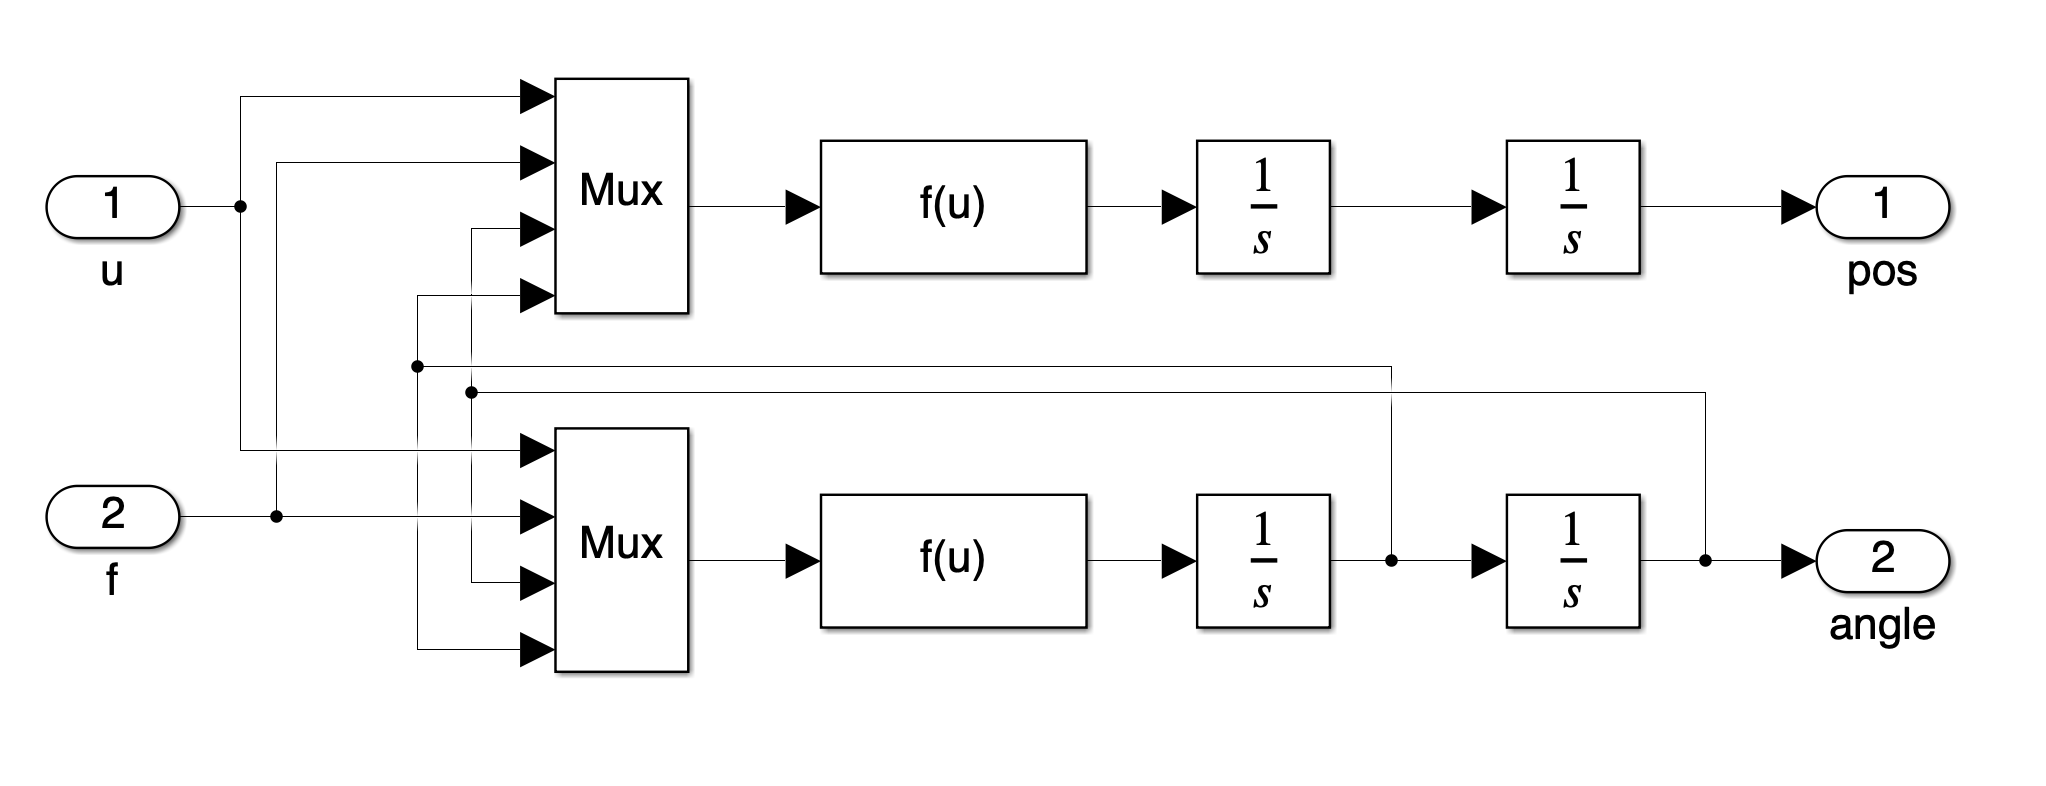
\includegraphics[width=0.8\textwidth]{media/scheme_unlinear.png}
    \caption{Схема блока нелинейной модели системы}
    \label{fig:scheme_unlinear}
\end{figure}
Уравнения в блоках \texttt{fcn} представляют собой уравнения (\ref{eq:nonlinear_model}) системы. 

\begin{figure}[ht!]
    \centering
    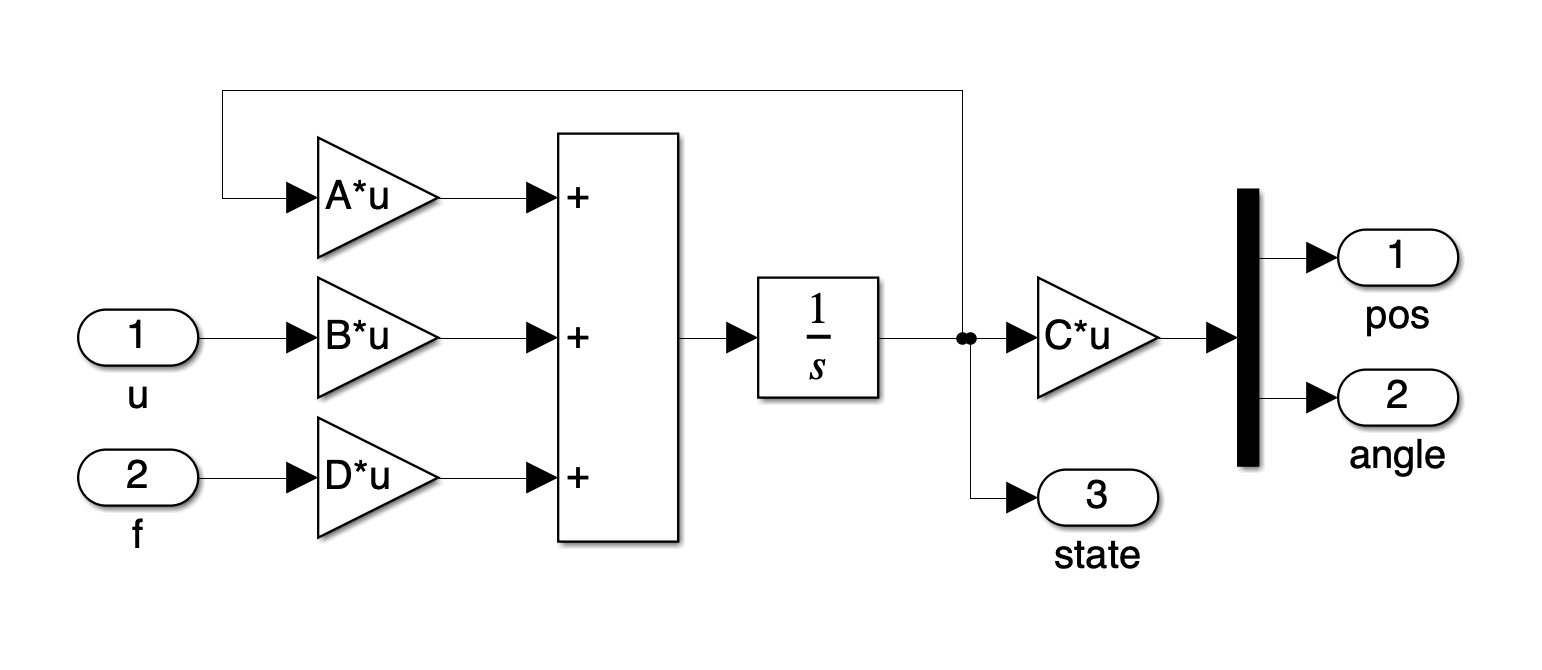
\includegraphics[width=0.8\textwidth]{media/scheme_linear.png}
    \caption{Схема блока линейной модели системы}
    \label{fig:scheme_linear}
\end{figure}

Проведем моделирование свободного движения системы в отсутствии внешнего 
возмущения с различными начальными условиями: будем изменять 
начальное положение маятника (его отклонение от верхнего положения равновесия), все остальные параметры 
системы оставим равными нулю. В качестве начального условия выберем угол отклонения маятника из множества 
$[0, 0.1, -0.1, 0.3, \nicefrac{\pi}{2}, \pi]$. Результаты моделирования представлены на
рисунке \ref{fig:free_motion_nonlinear} и \ref{fig:free_motion_linear}.
\begin{figure}[ht!]
    \centering
    \begin{subfigure}[b]{0.45\textwidth}
        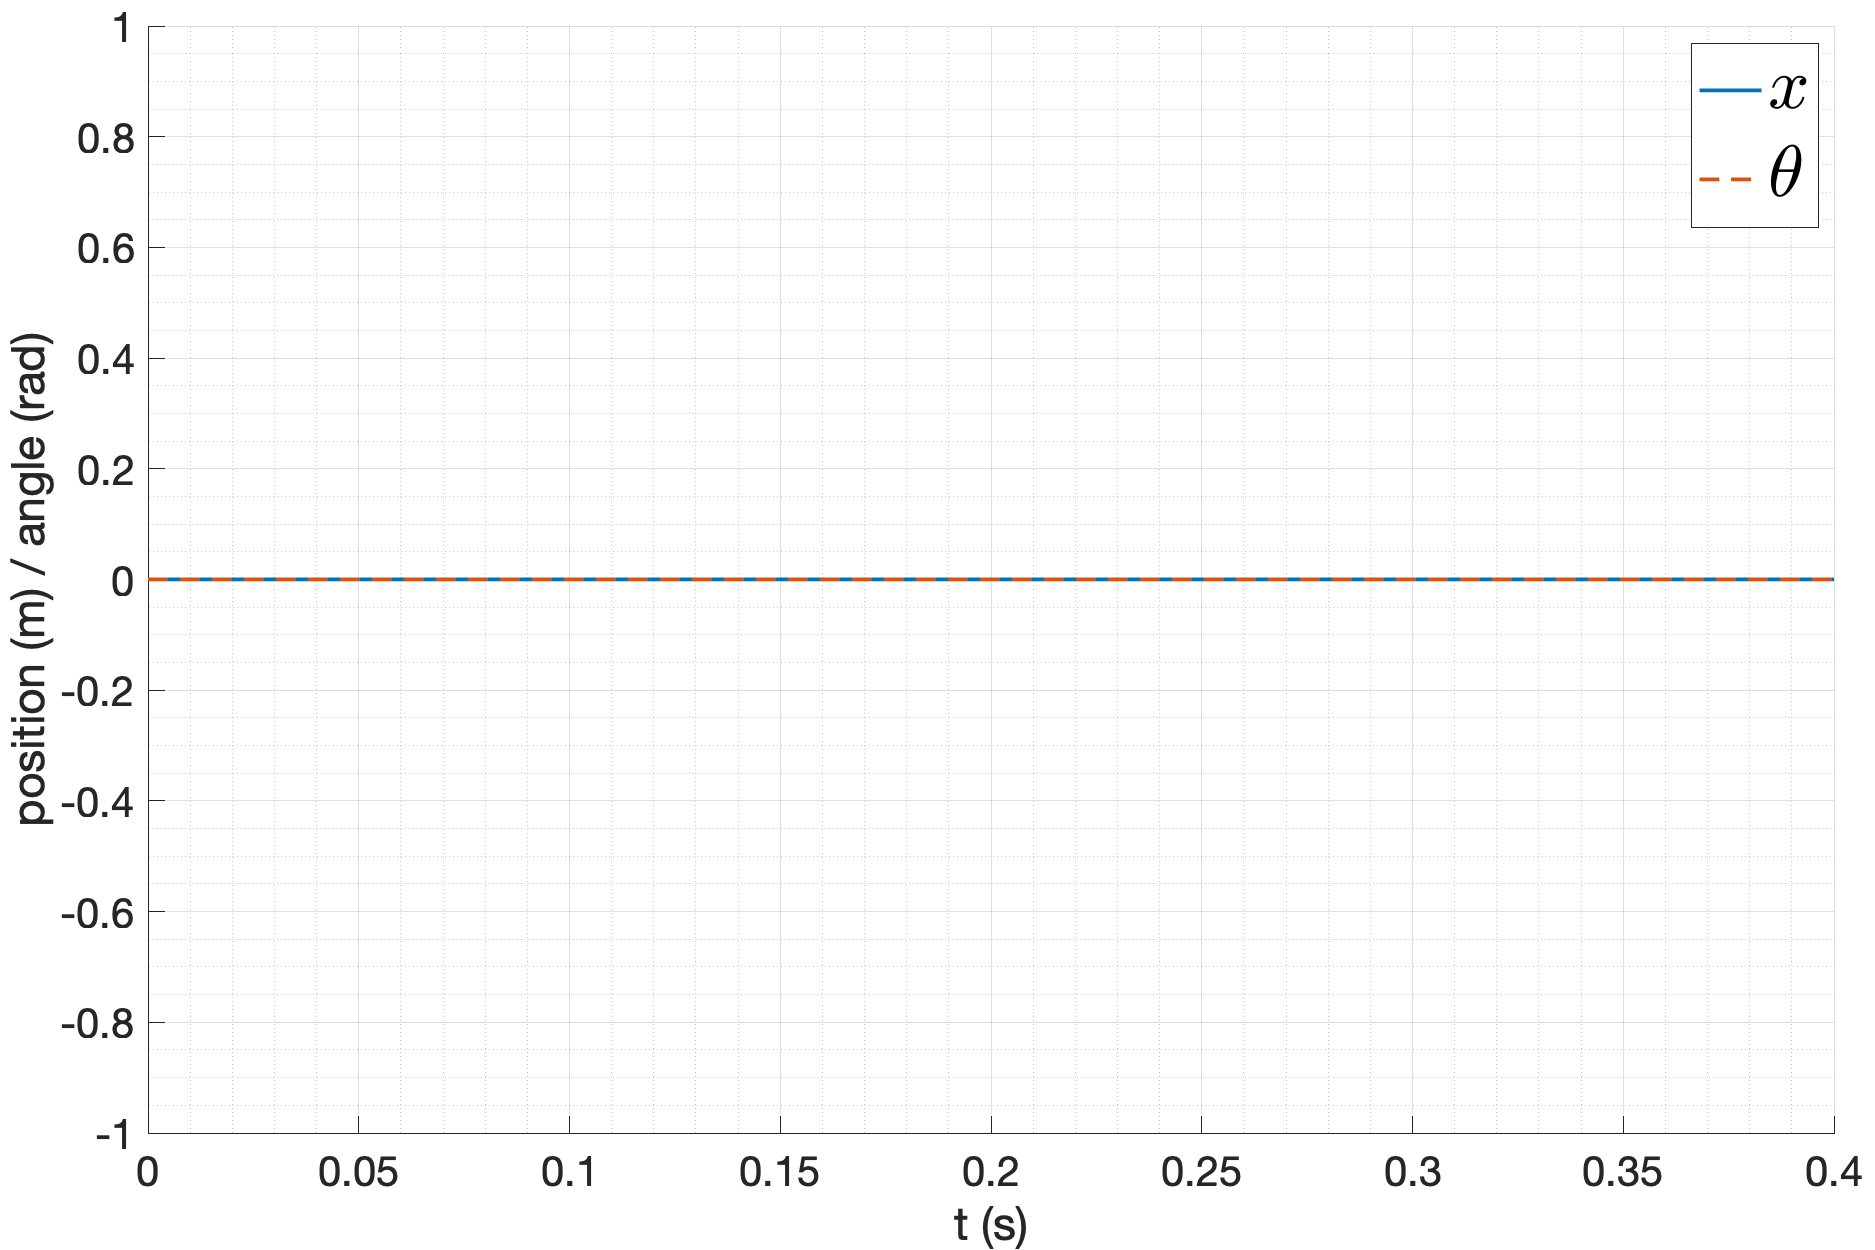
\includegraphics[width=\textwidth]{media/plots/free_motion/nonlin_1.png}
        \caption{$\theta_0 = 0$}
  \end{subfigure}
    \begin{subfigure}[b]{0.45\textwidth}
        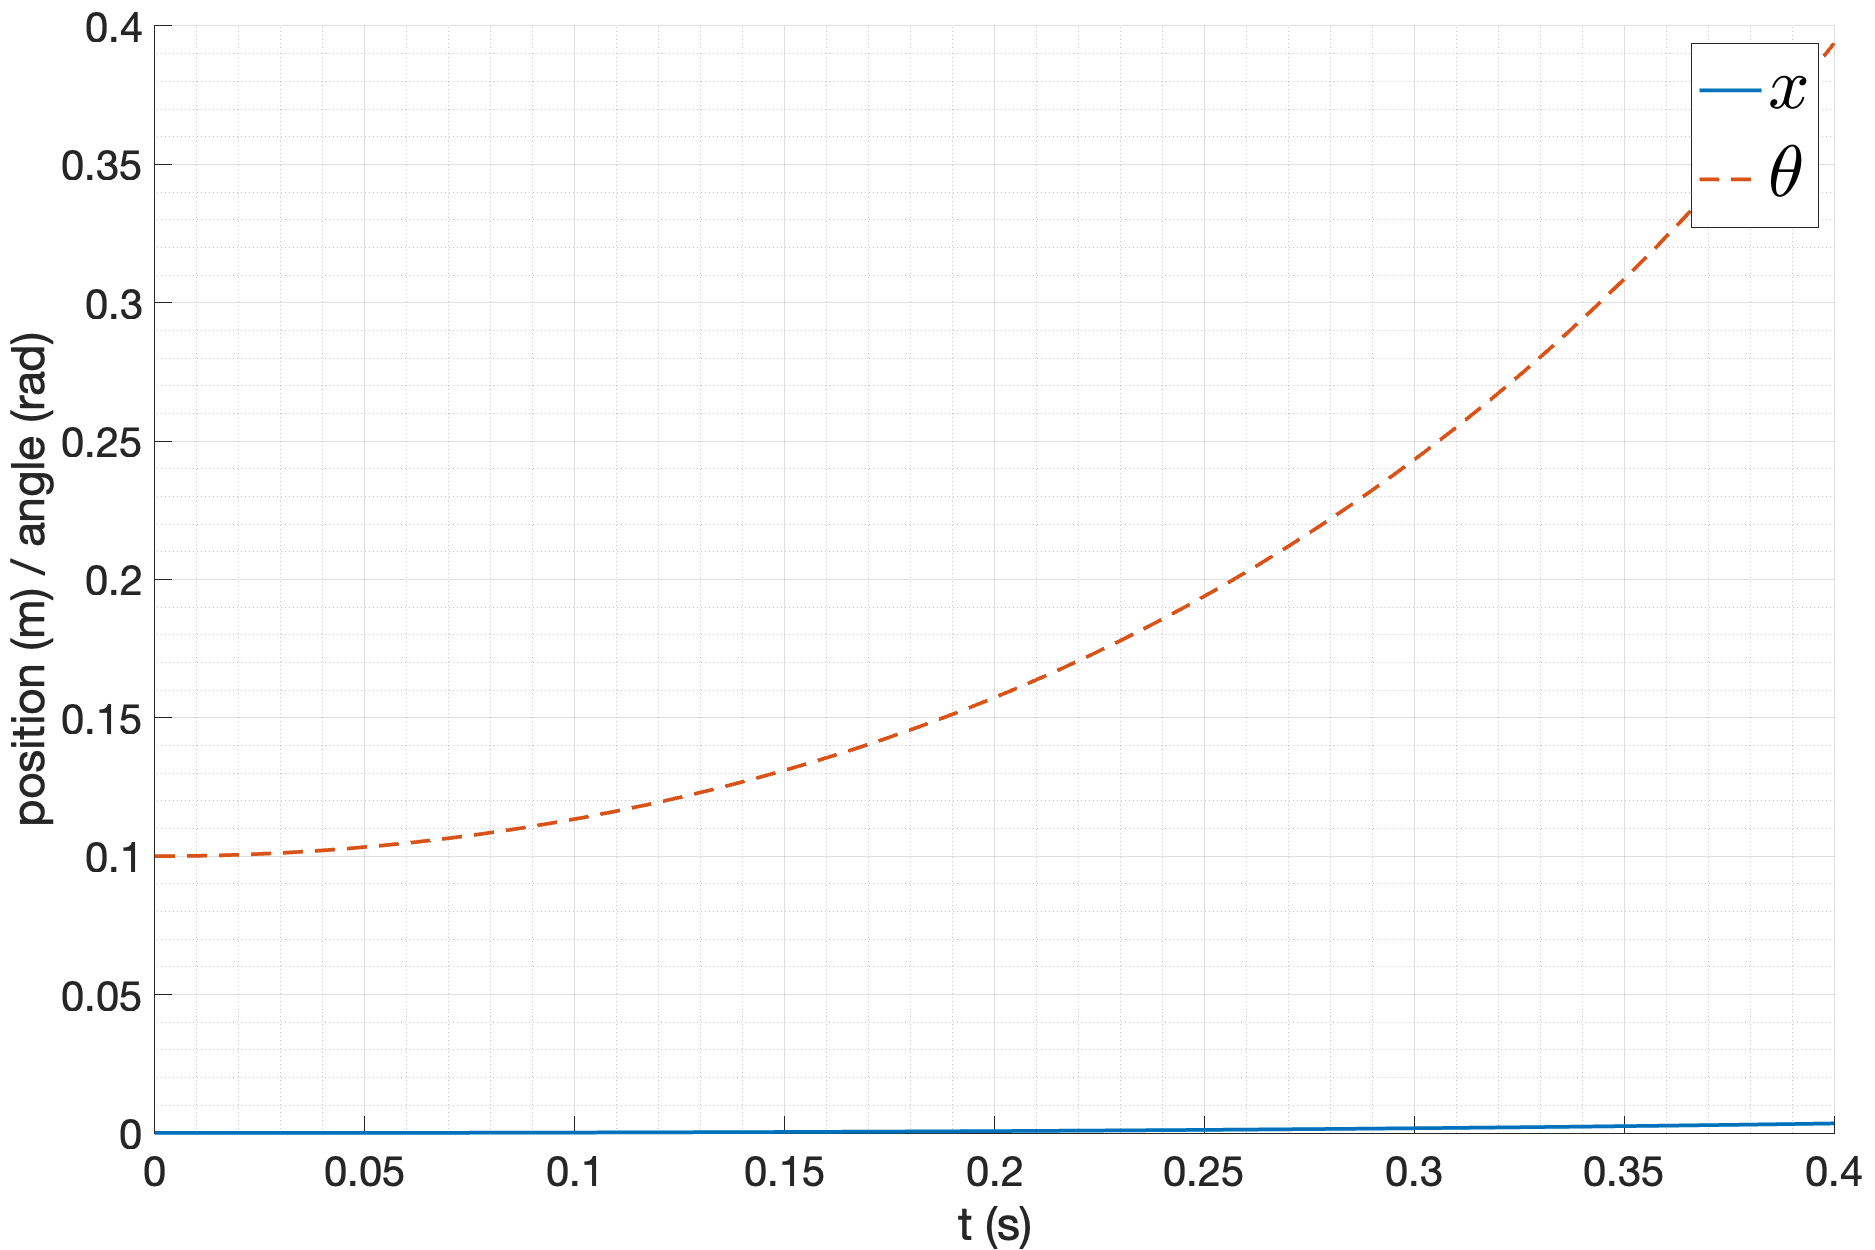
\includegraphics[width=\textwidth]{media/plots/free_motion/nonlin_2.png}
        \caption{$\theta_0 = 0.1$}
    \end{subfigure}
    \begin{subfigure}[b]{0.45\textwidth}
        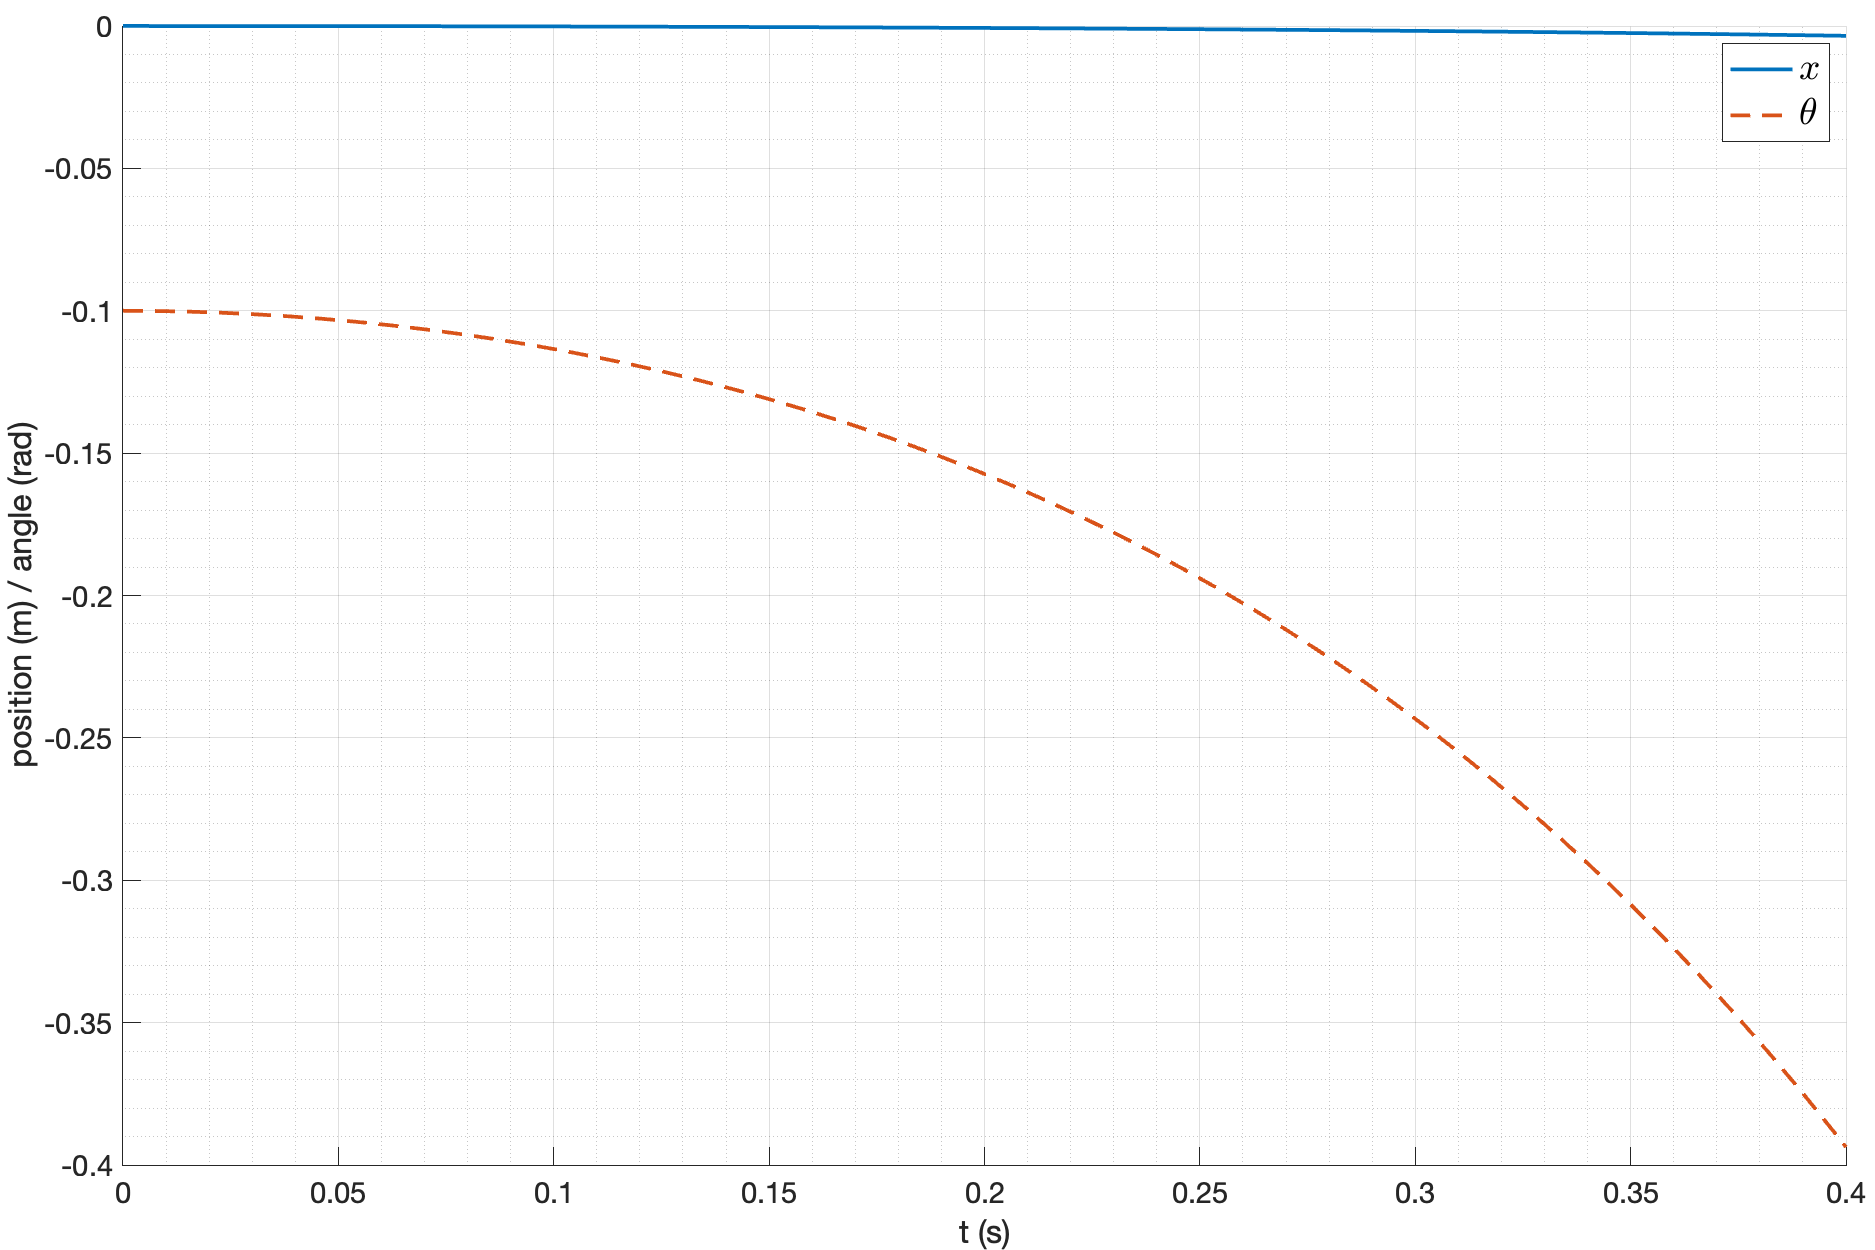
\includegraphics[width=\textwidth]{media/plots/free_motion/nonlin_3.png}
        \caption{$\theta_0 = -0.1$}
    \end{subfigure}
    \begin{subfigure}[b]{0.45\textwidth}
        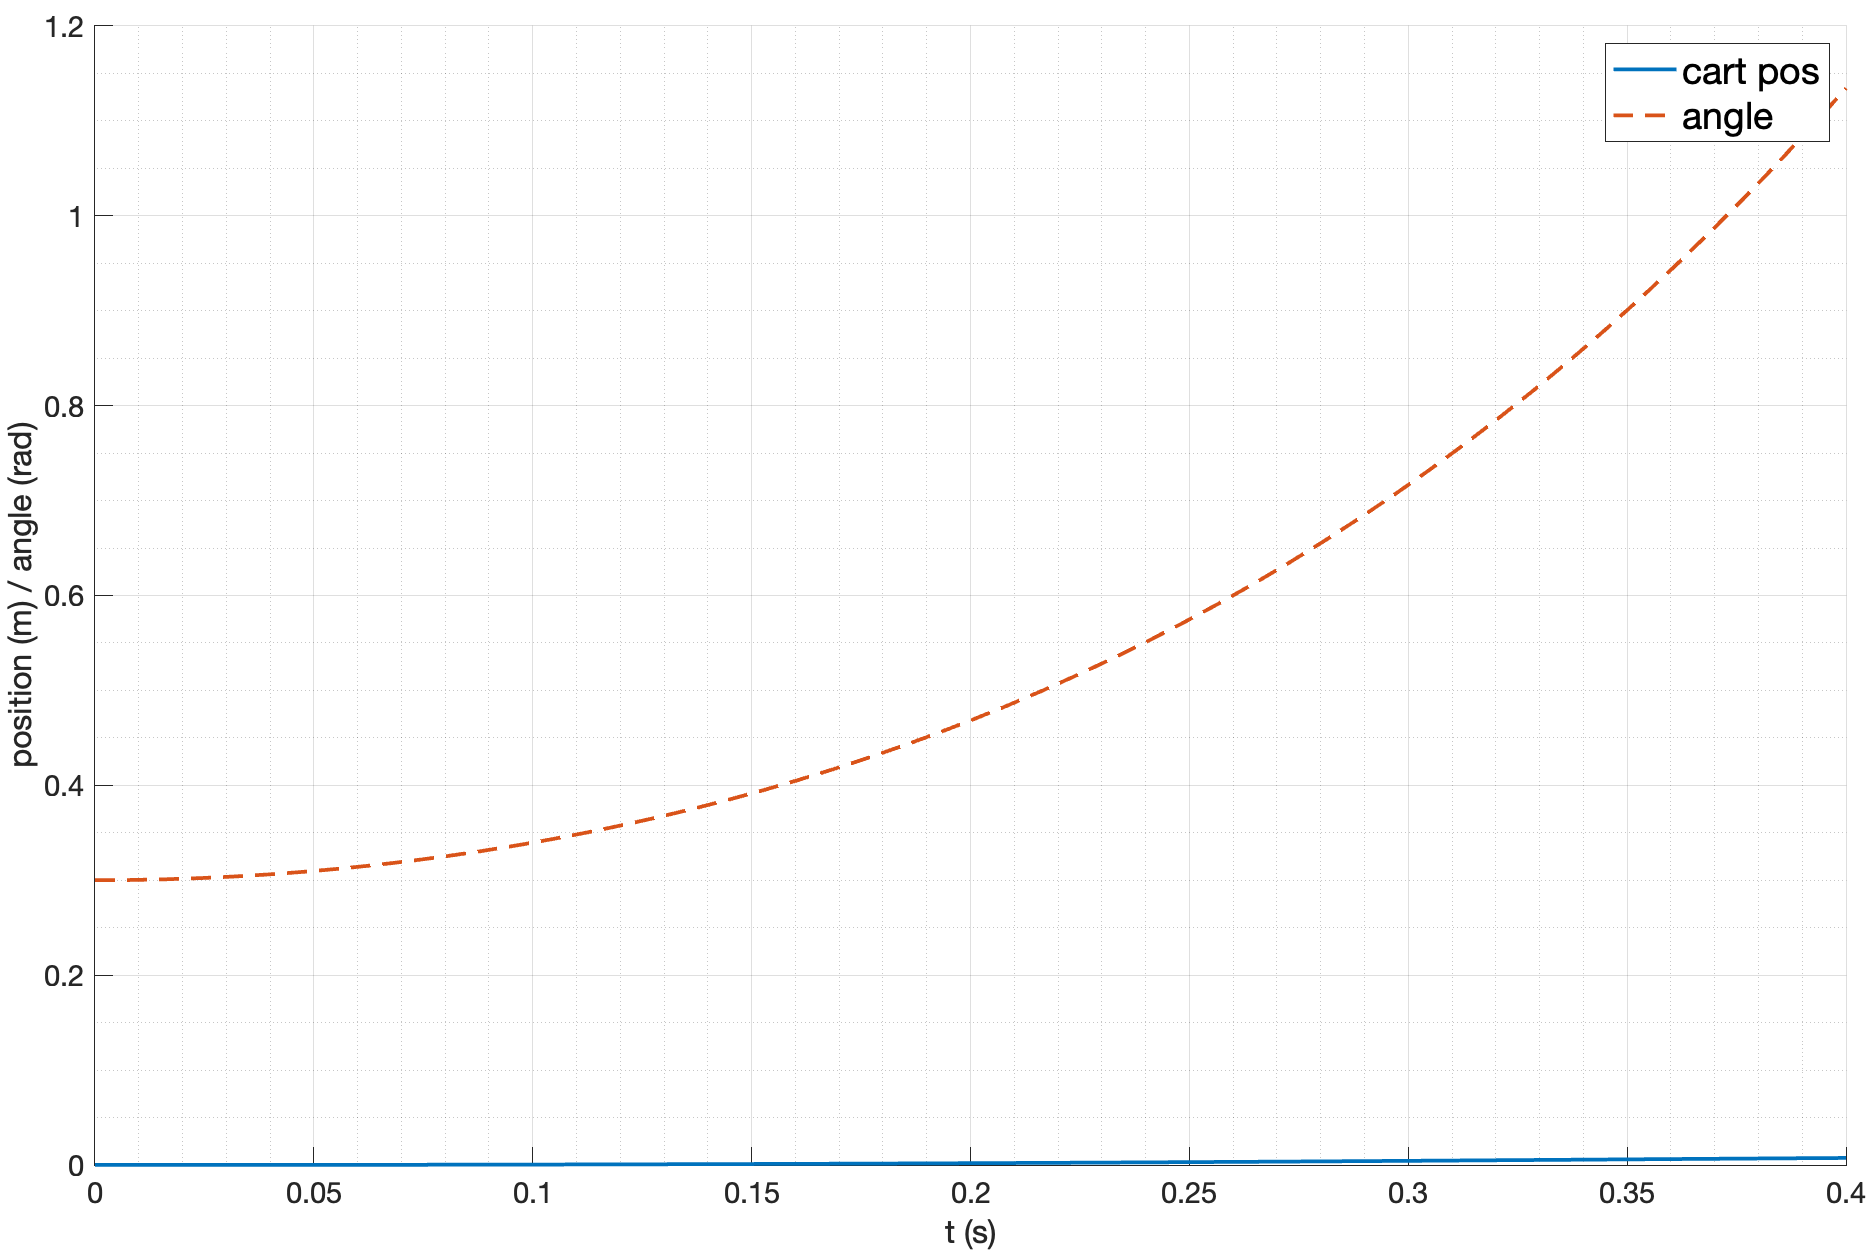
\includegraphics[width=\textwidth]{media/plots/free_motion/nonlin_4.png}
        \caption{$\theta_0 = 0.3$}
    \end{subfigure}
    \begin{subfigure}[b]{0.45\textwidth}
        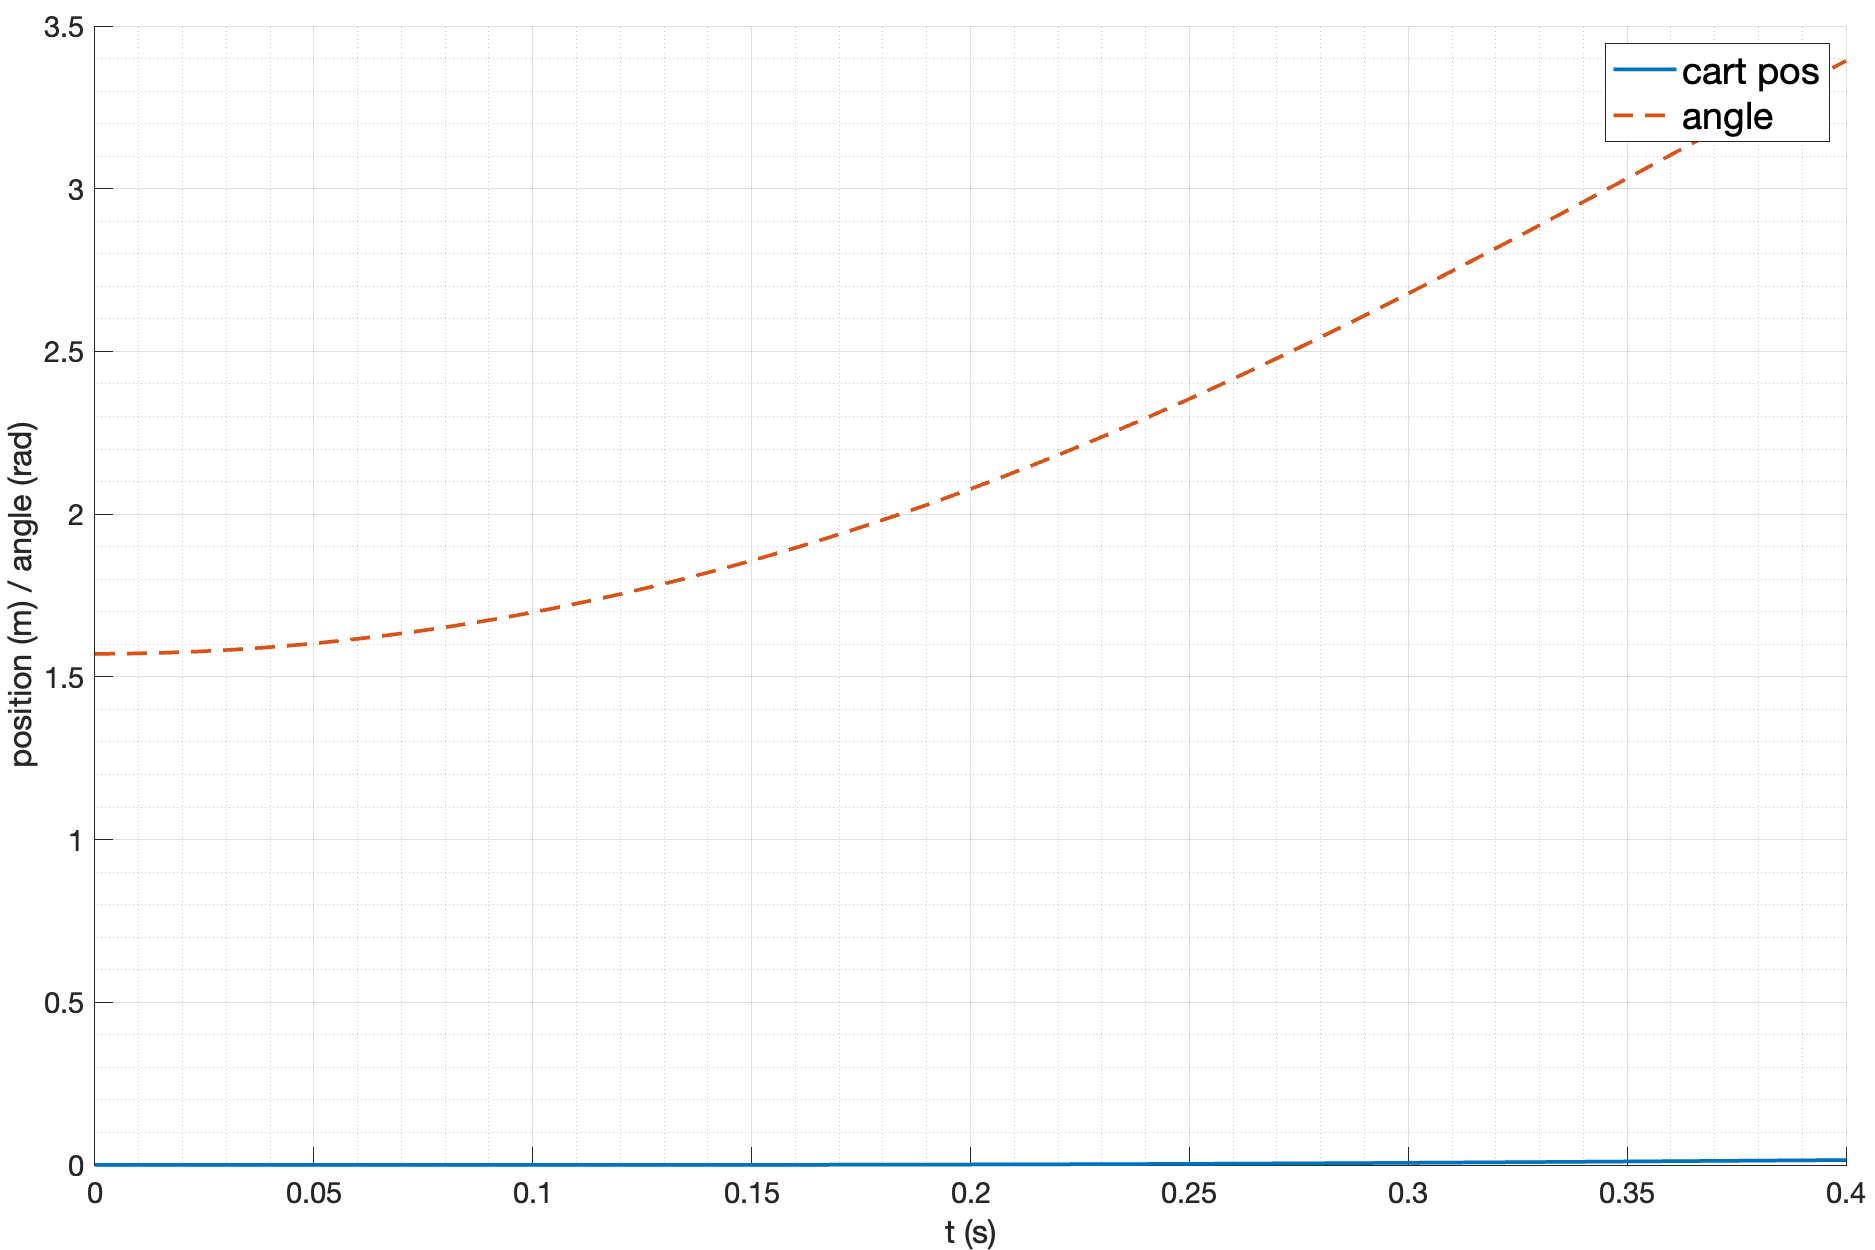
\includegraphics[width=\textwidth]{media/plots/free_motion/nonlin_5.png}
        \caption{$\theta_0 = \frac{\pi}{2}$}
    \end{subfigure}
    \begin{subfigure}[b]{0.45\textwidth}
        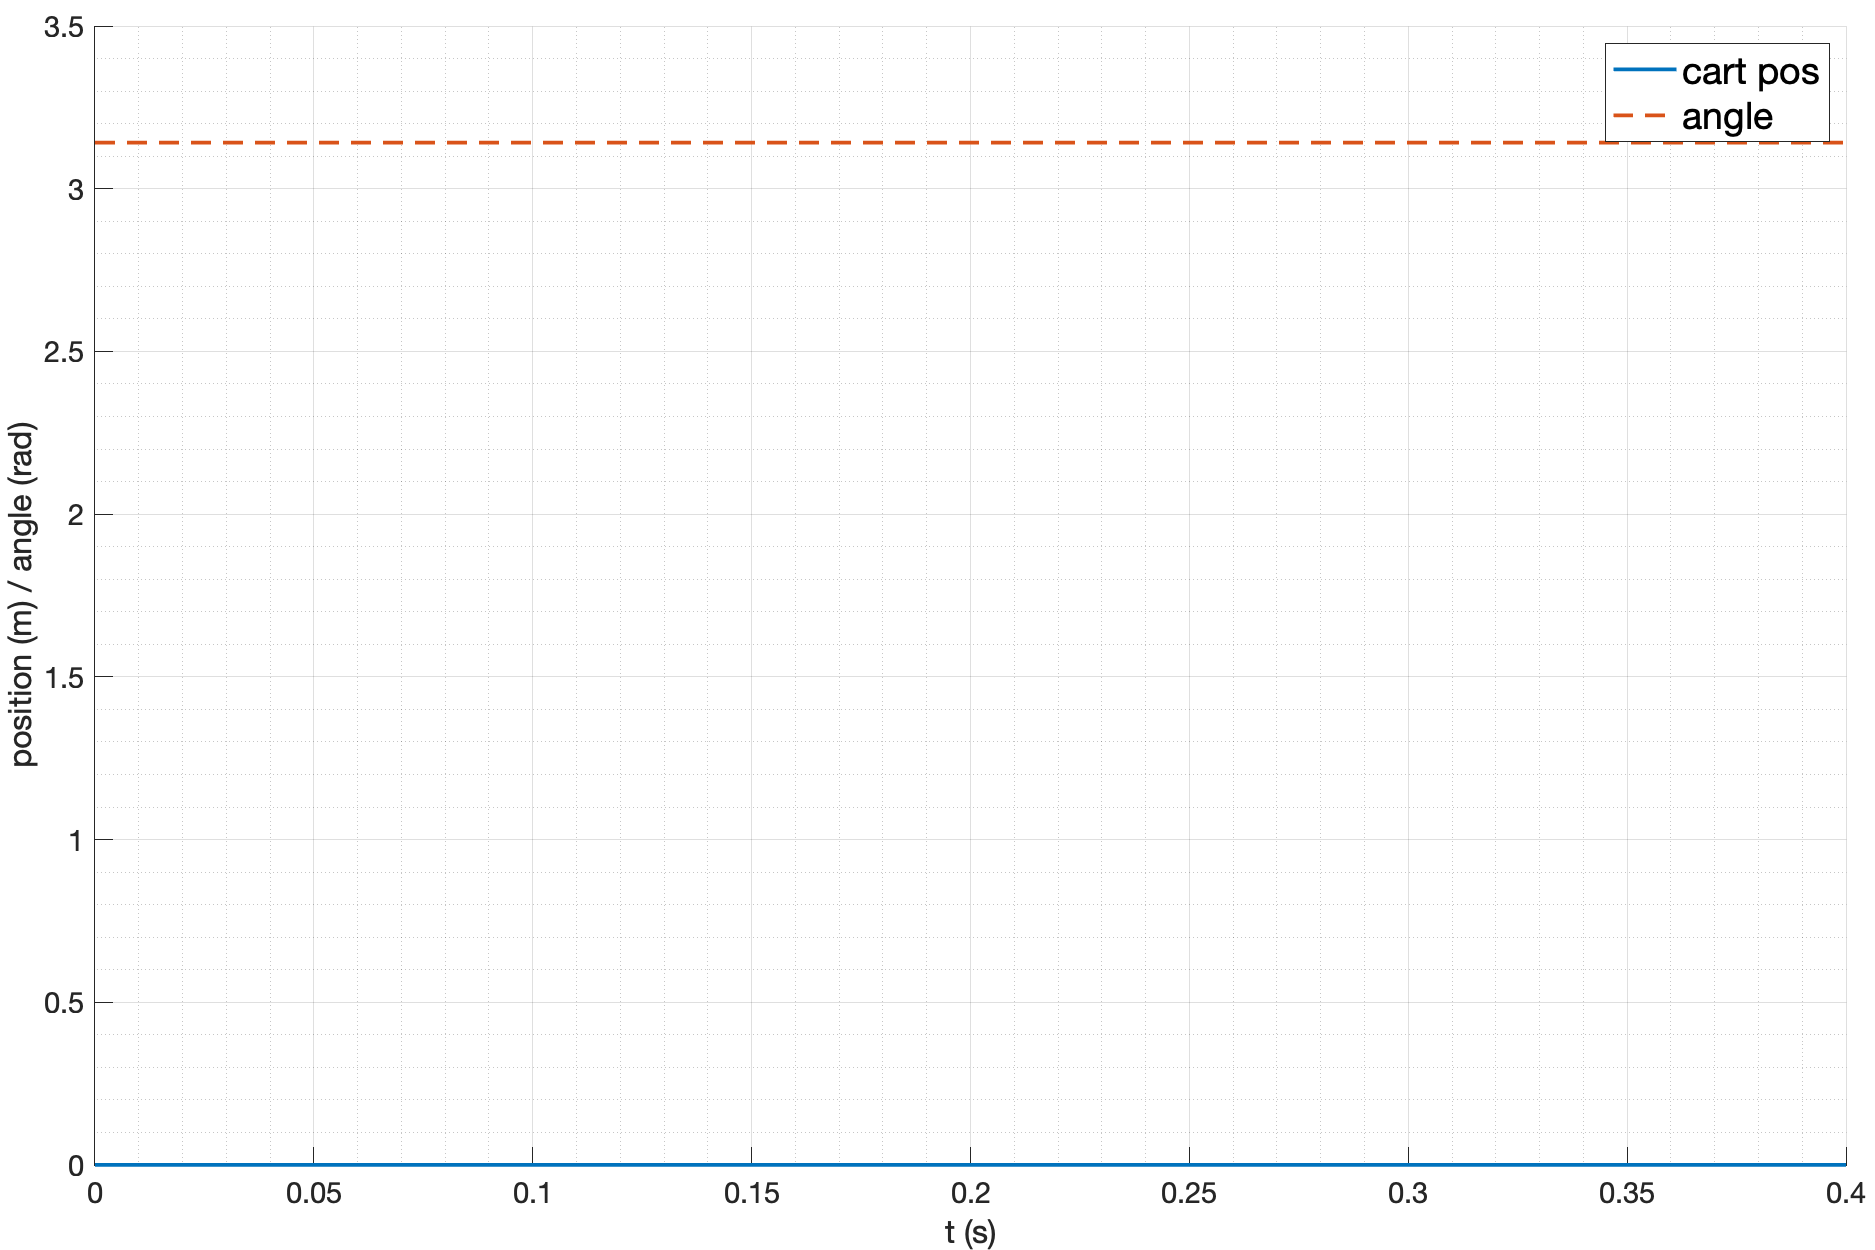
\includegraphics[width=\textwidth]{media/plots/free_motion/nonlin_6.png}
        \caption{$\theta_0 = \pi$}
    \end{subfigure}
    \caption{Свободное движение маятника (нелинейная модель)}
    \label{fig:free_motion_nonlinear}
\end{figure}

\begin{figure}[ht!]
    \centering
    \begin{subfigure}[b]{0.45\textwidth}
        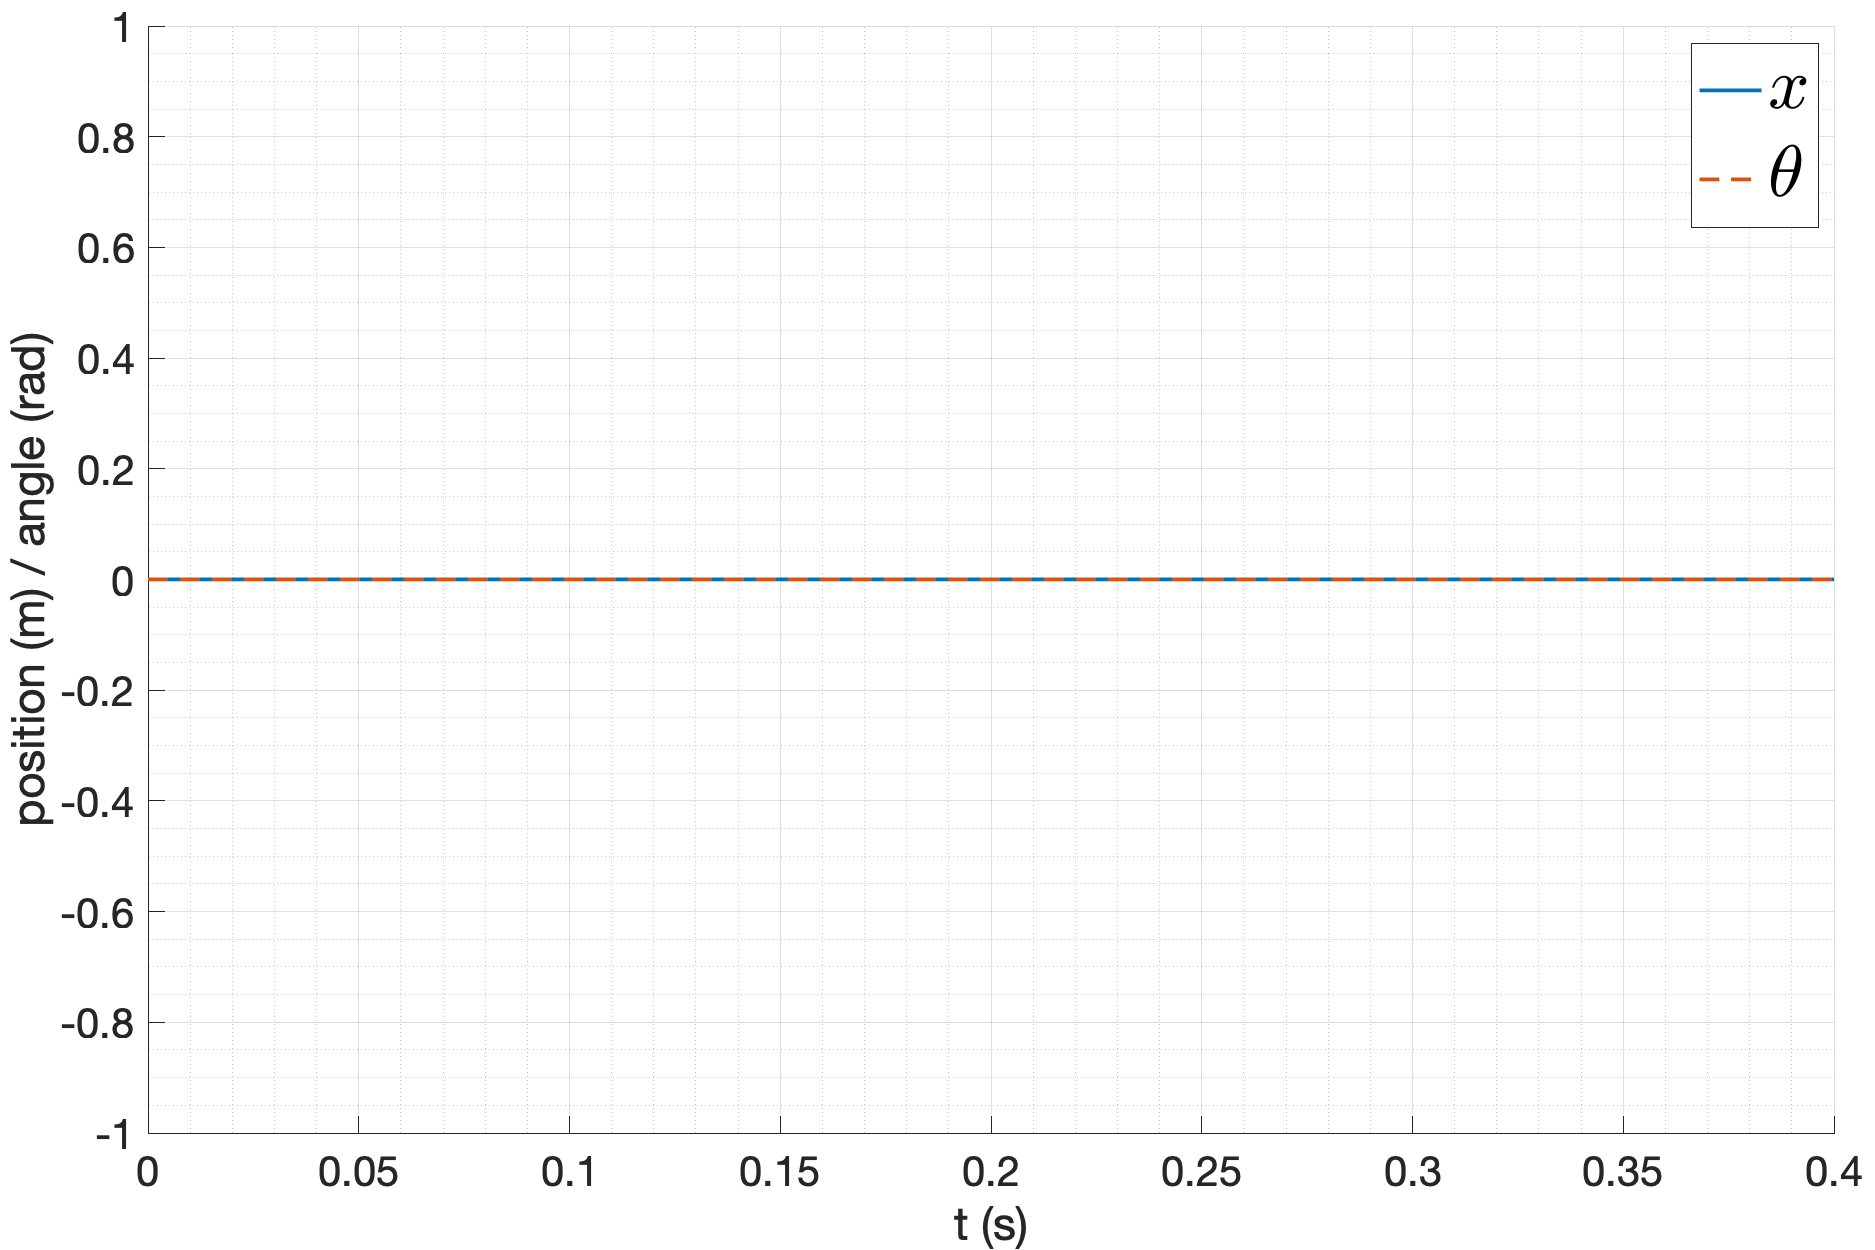
\includegraphics[width=\textwidth]{media/plots/free_motion/lin_1.png}
        \caption{$\theta_0 = 0$}
  \end{subfigure}
    \begin{subfigure}[b]{0.45\textwidth}
        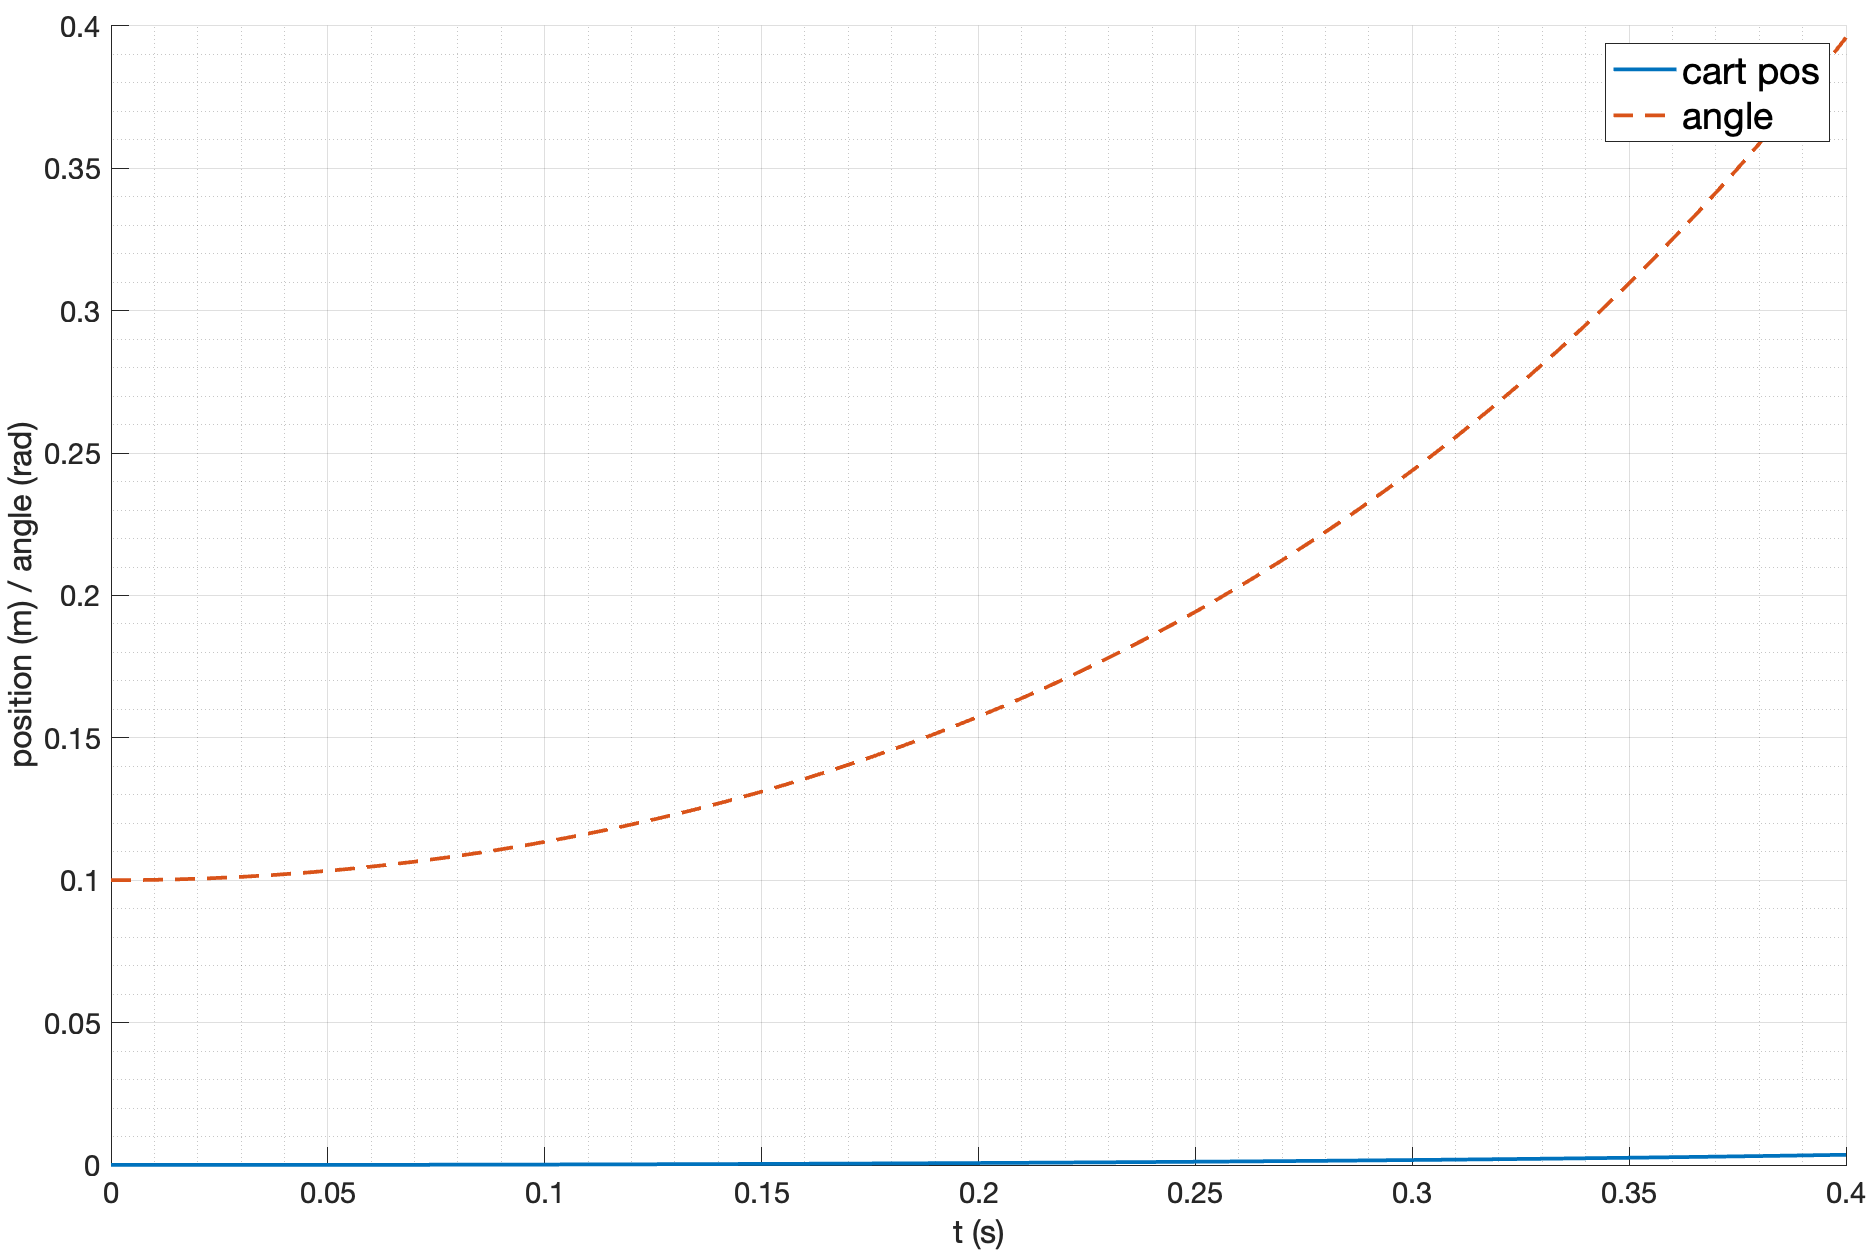
\includegraphics[width=\textwidth]{media/plots/free_motion/lin_2.png}
        \caption{$\theta_0 = 0.1$}
    \end{subfigure}
    \begin{subfigure}[b]{0.45\textwidth}
        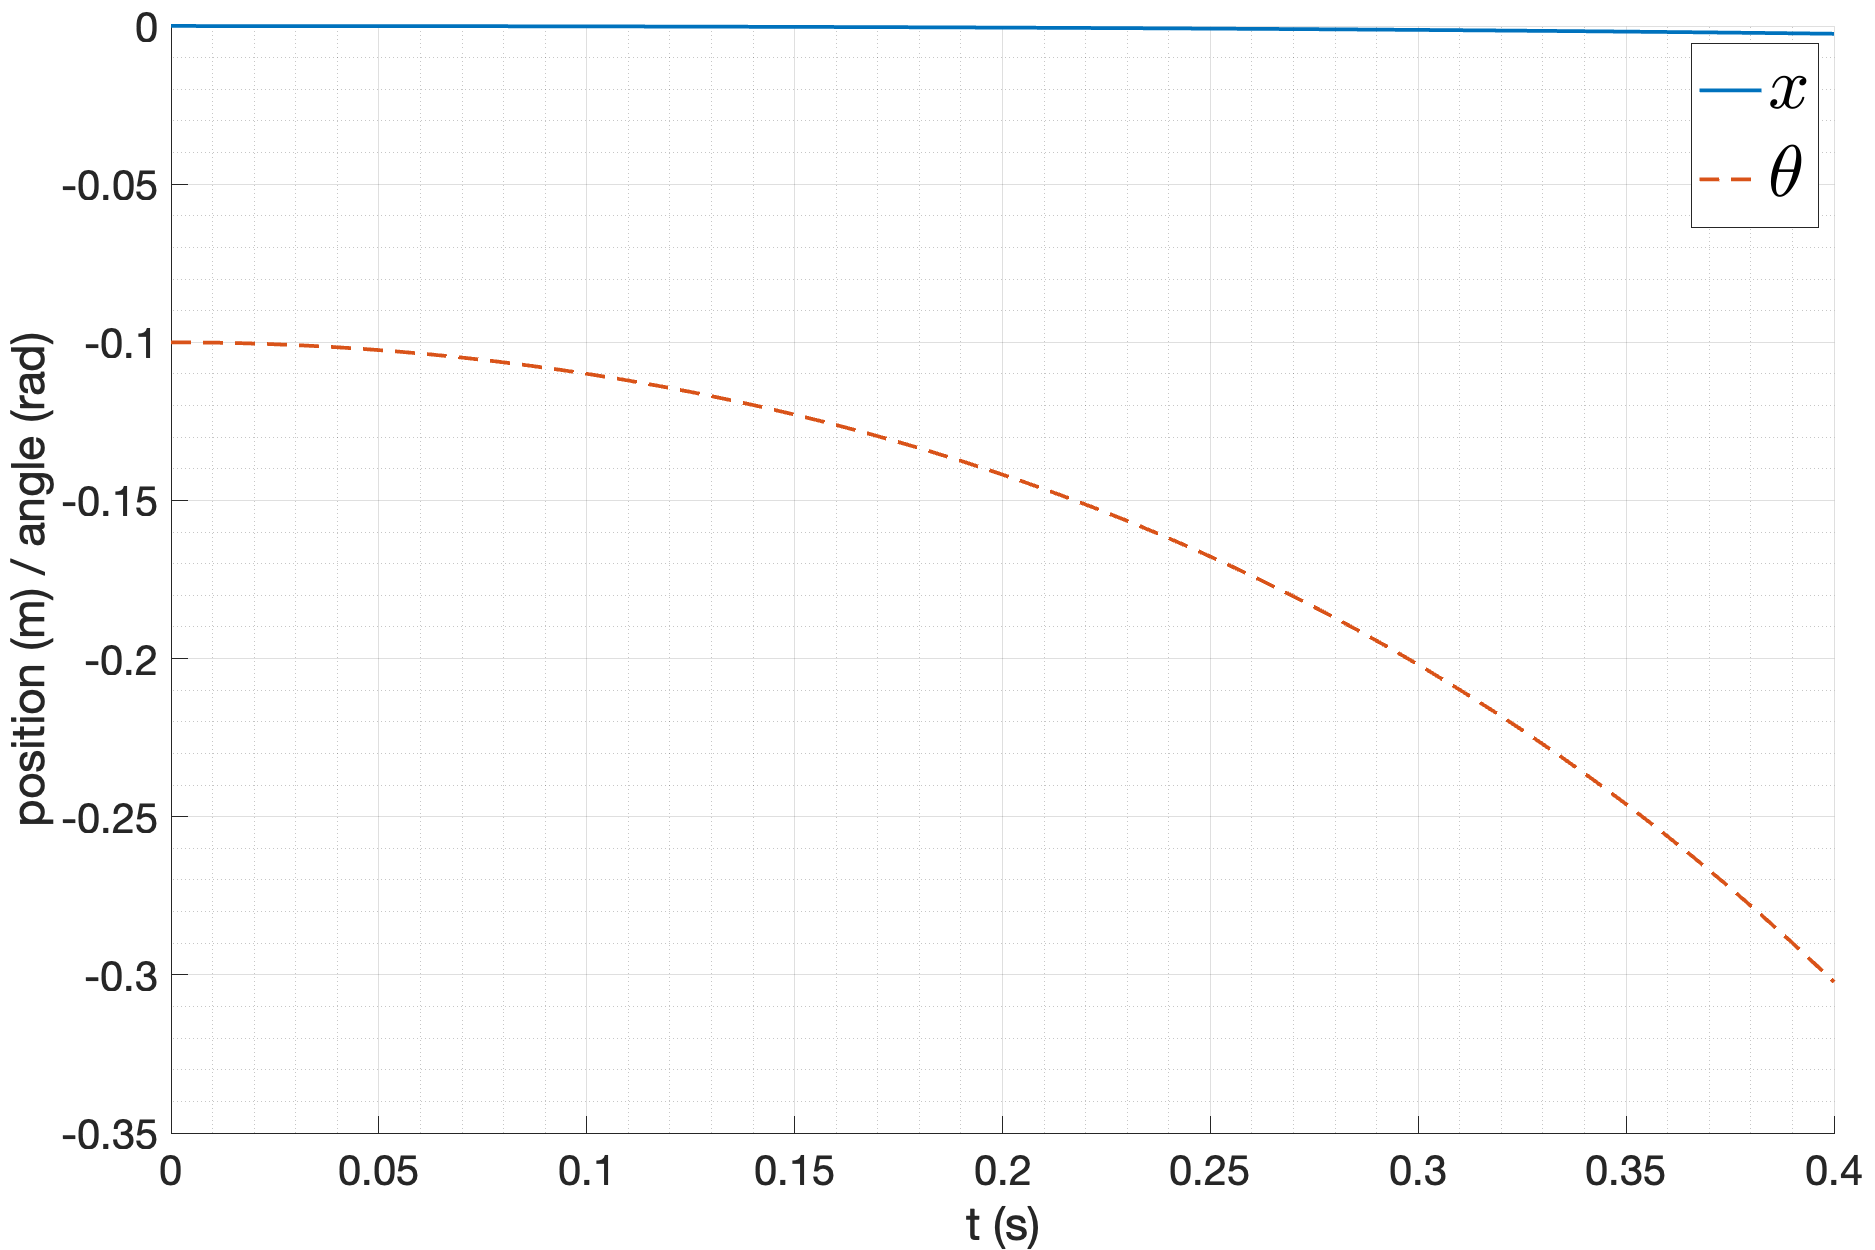
\includegraphics[width=\textwidth]{media/plots/free_motion/lin_3.png}
        \caption{$\theta_0 = -0.1$}
    \end{subfigure}
    \begin{subfigure}[b]{0.45\textwidth}
        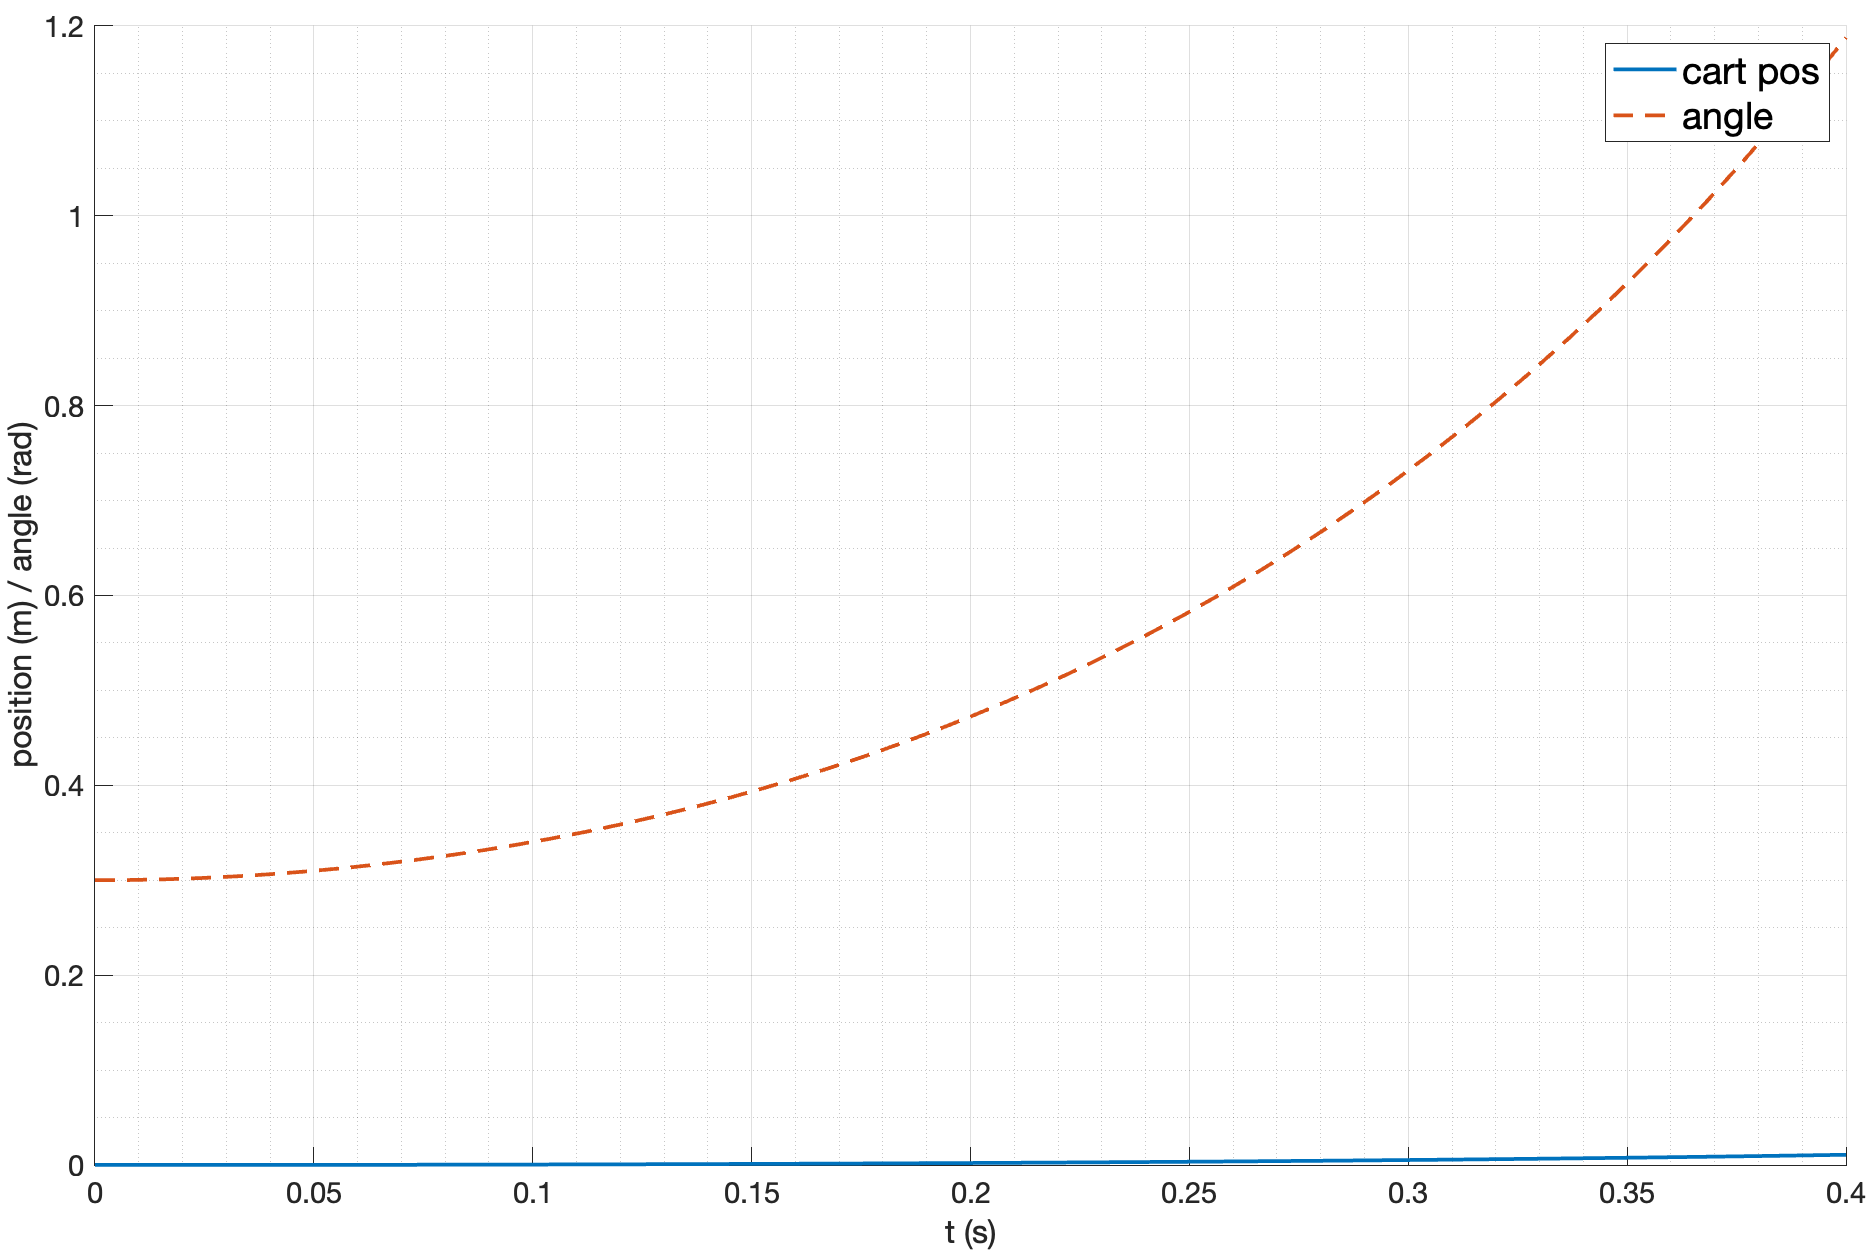
\includegraphics[width=\textwidth]{media/plots/free_motion/lin_4.png}
        \caption{$\theta_0 = 0.3$}
    \end{subfigure}
    \begin{subfigure}[b]{0.45\textwidth}
        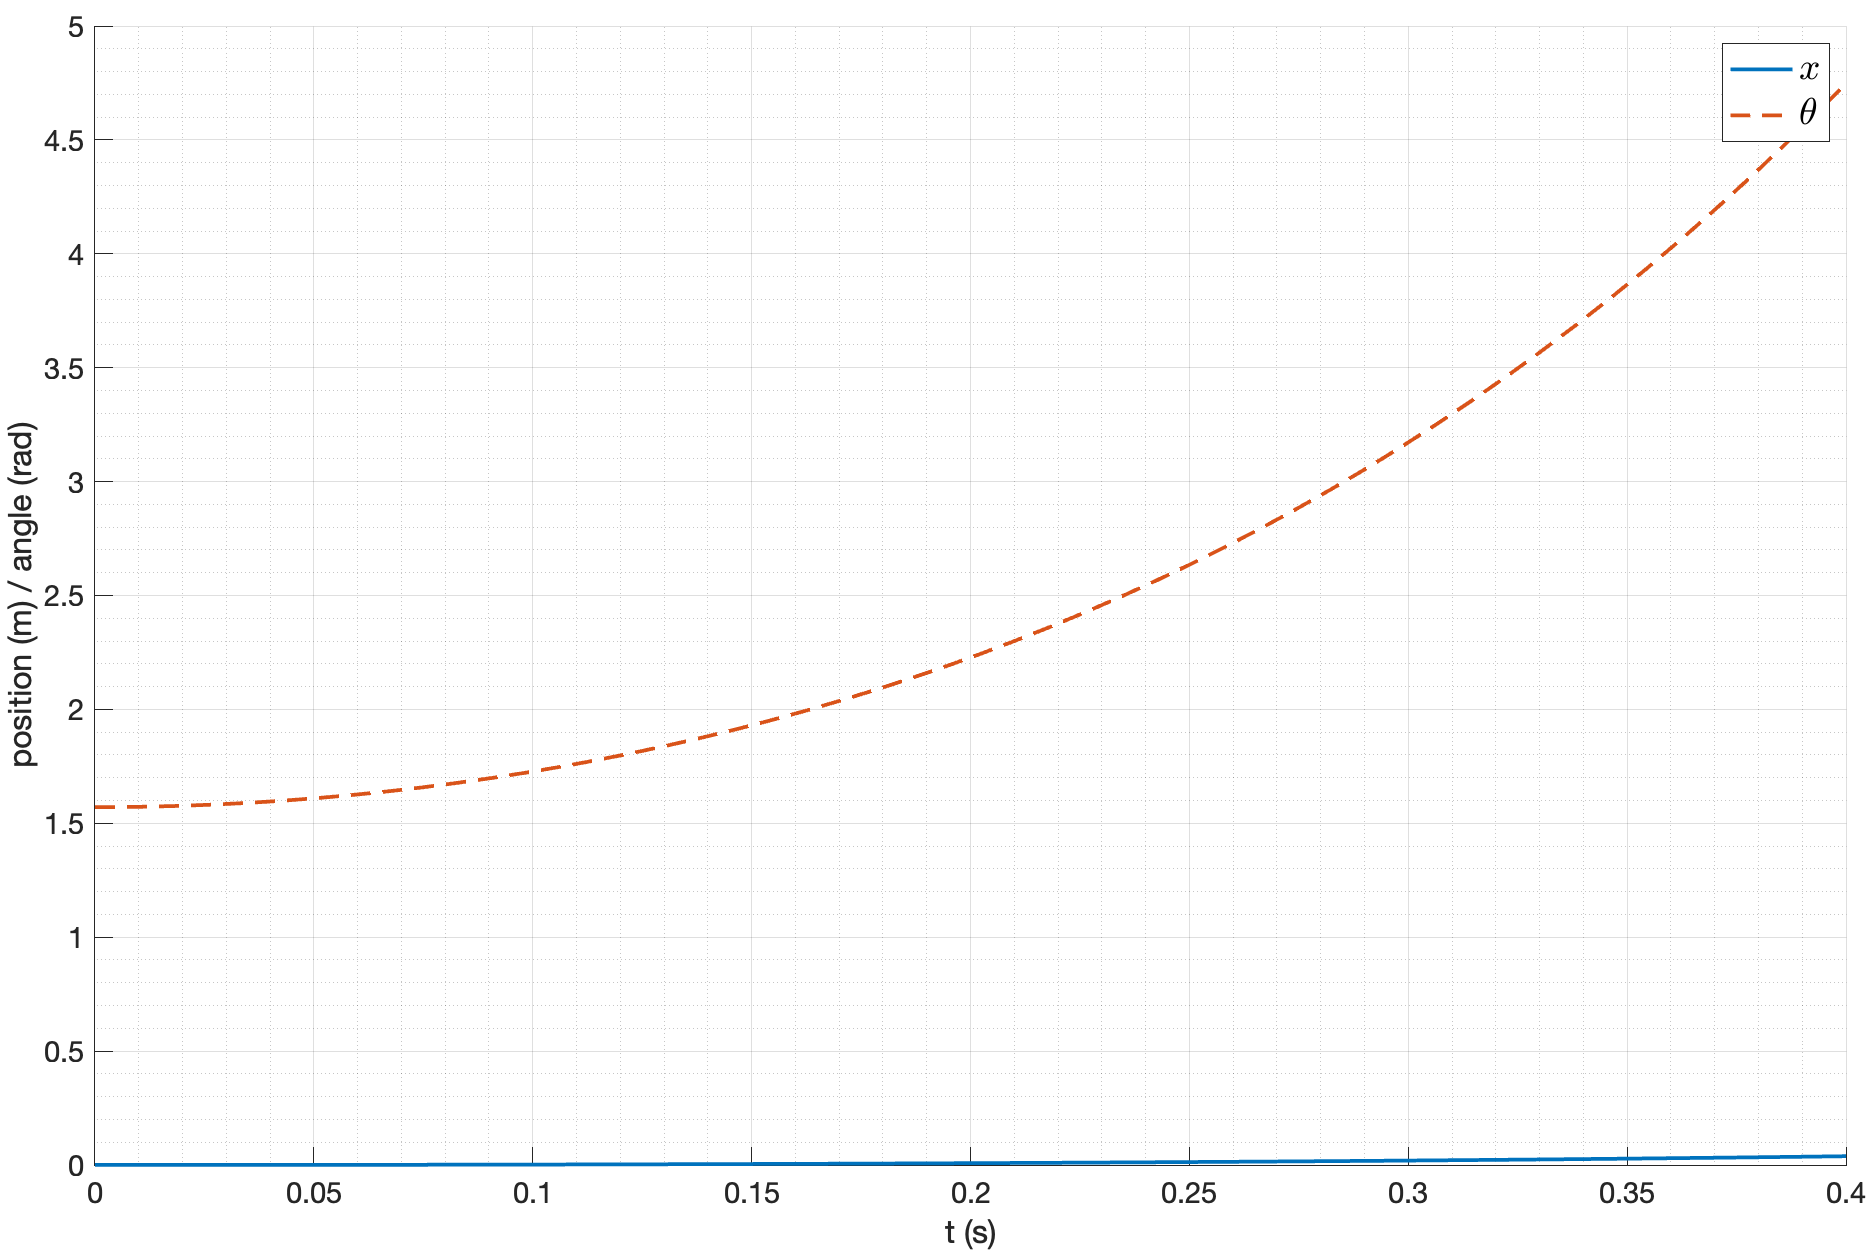
\includegraphics[width=\textwidth]{media/plots/free_motion/lin_5.png}
        \caption{$\theta_0 = \frac{\pi}{2}$}
    \end{subfigure}
    \begin{subfigure}[b]{0.45\textwidth}
        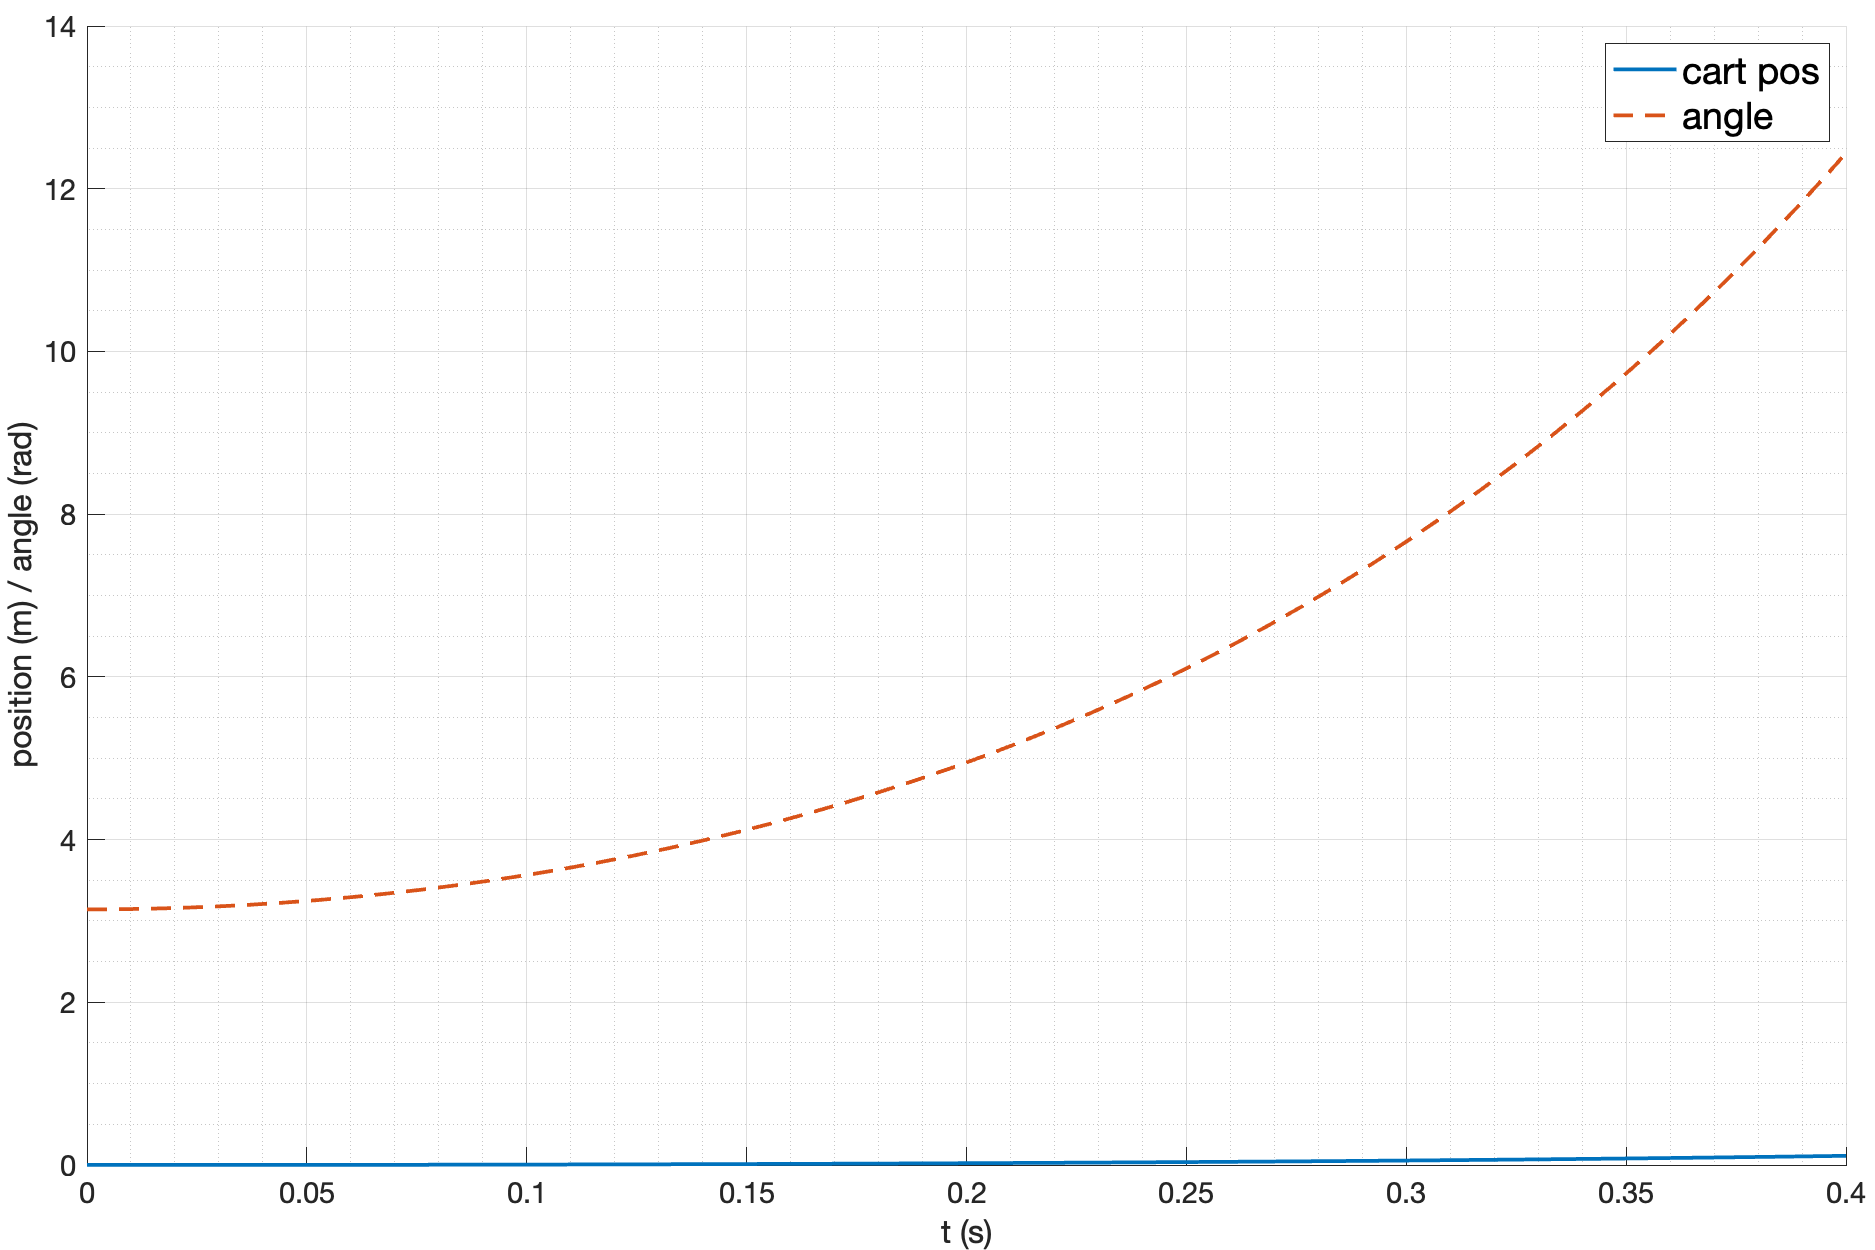
\includegraphics[width=\textwidth]{media/plots/free_motion/lin_6.png}
        \caption{$\theta_0 = \pi$}
    \end{subfigure}
    \caption{Свободное движение маятника (линеаризованная модель)}
    \label{fig:free_motion_linear}
\end{figure}

На рисунках \ref{fig:free_motion_nonlinear} и \ref{fig:free_motion_linear} видно, что при 
отсутствии отклонения от вертикального положения маятник остается в покое, 
при отклонении от вертикального положения маятник начинает движение, причем 
направление движения зависит от направления отклонения. При отклонении 
равным $\pi$, что соответствует нижнему положению равновесия, в случае нелинейной 
модели, остается неподвижным, в то время как в случае линеаризованной модели 
маятник начинает движение, что связано с тем, что линеаризация проводилась в окрестности
верхней точки равновесия, а не нижней. Сравним результаты моделирования
нелинейной и линеаризованной моделей. Графики различия движения приведены на
рисунке \ref{fig:free_motion_err}. 

\begin{figure}[ht!]
    \centering
    \begin{subfigure}[b]{0.45\textwidth}
        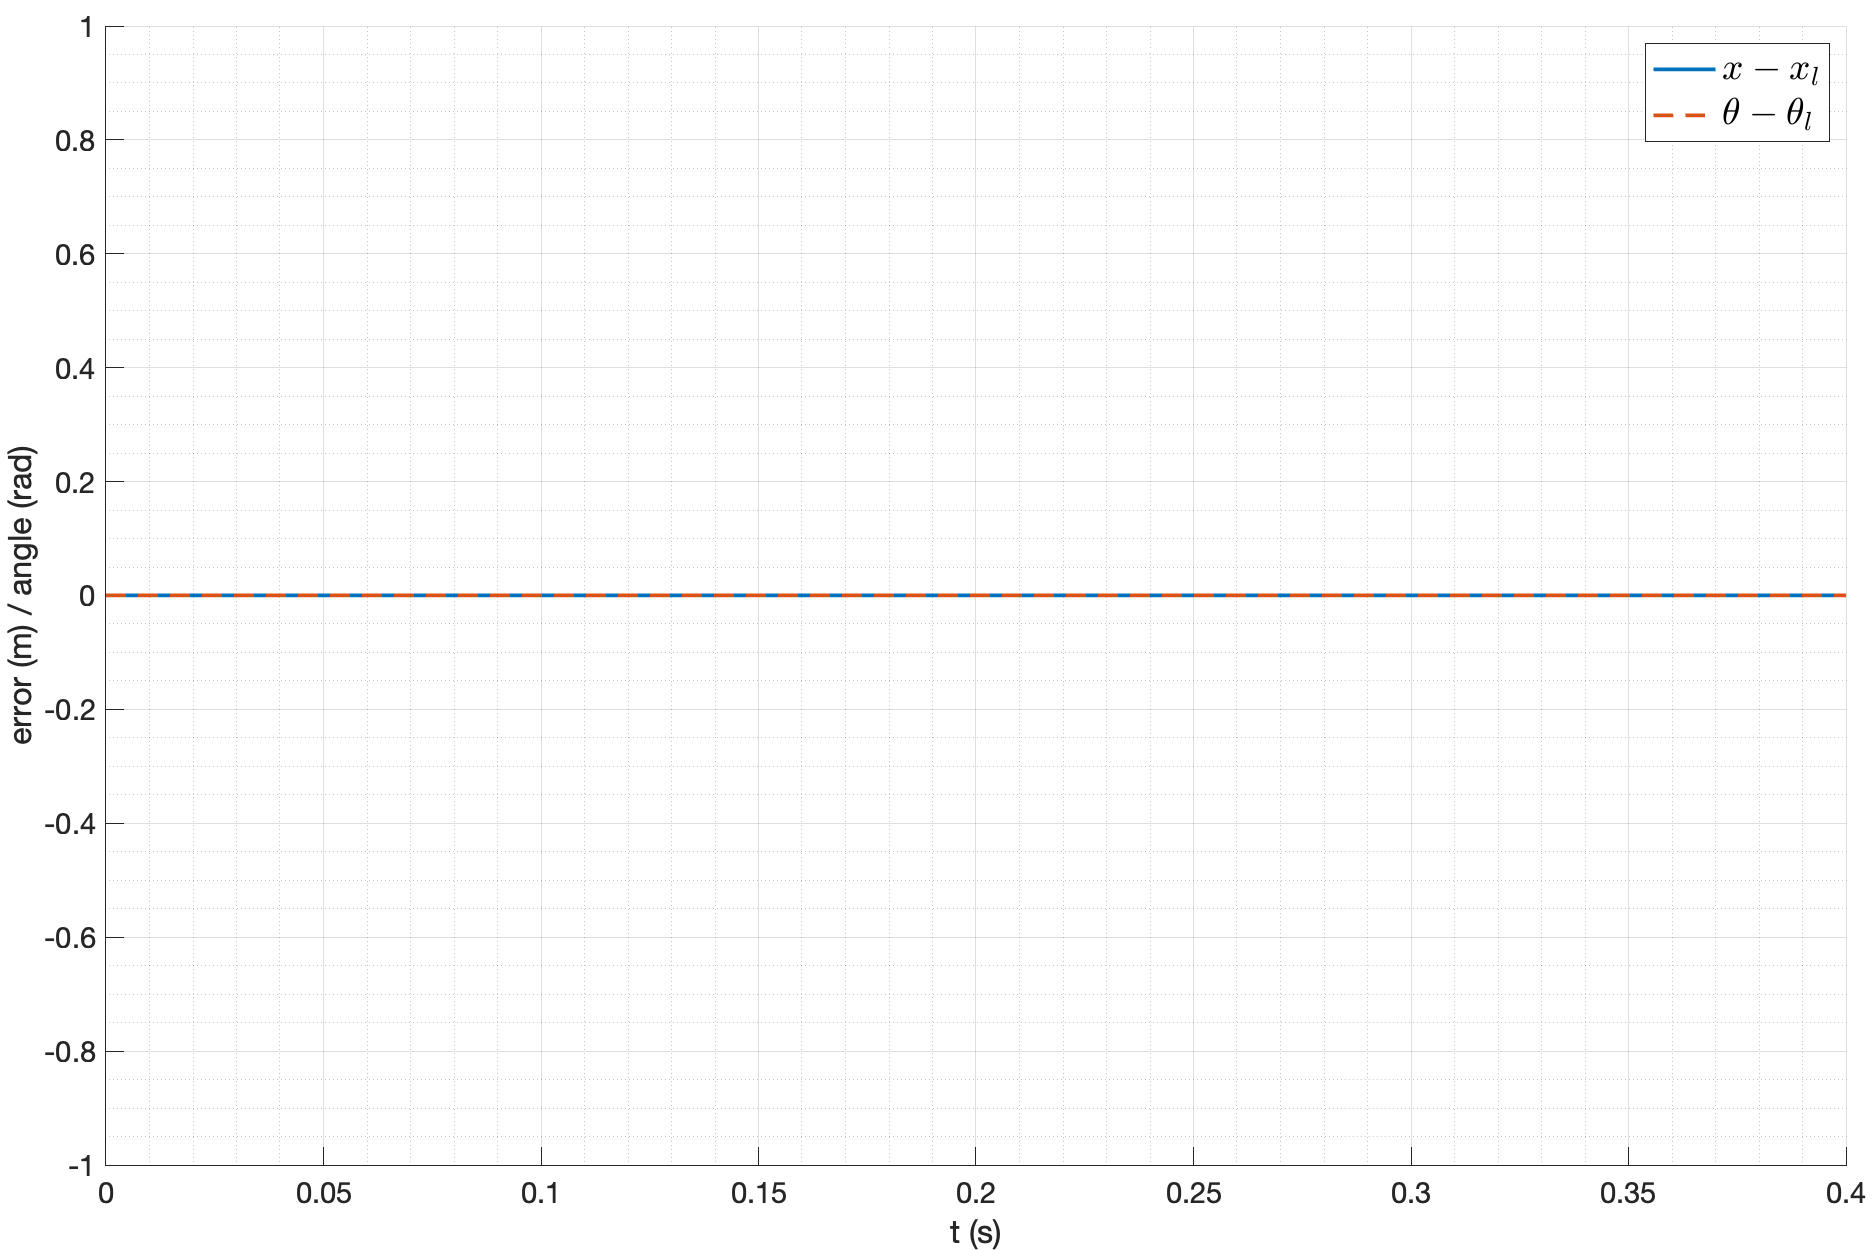
\includegraphics[width=\textwidth]{media/plots/free_motion/err_1.png}
        \caption{$\theta_0 = 0$}
  \end{subfigure}
    \begin{subfigure}[b]{0.45\textwidth}
        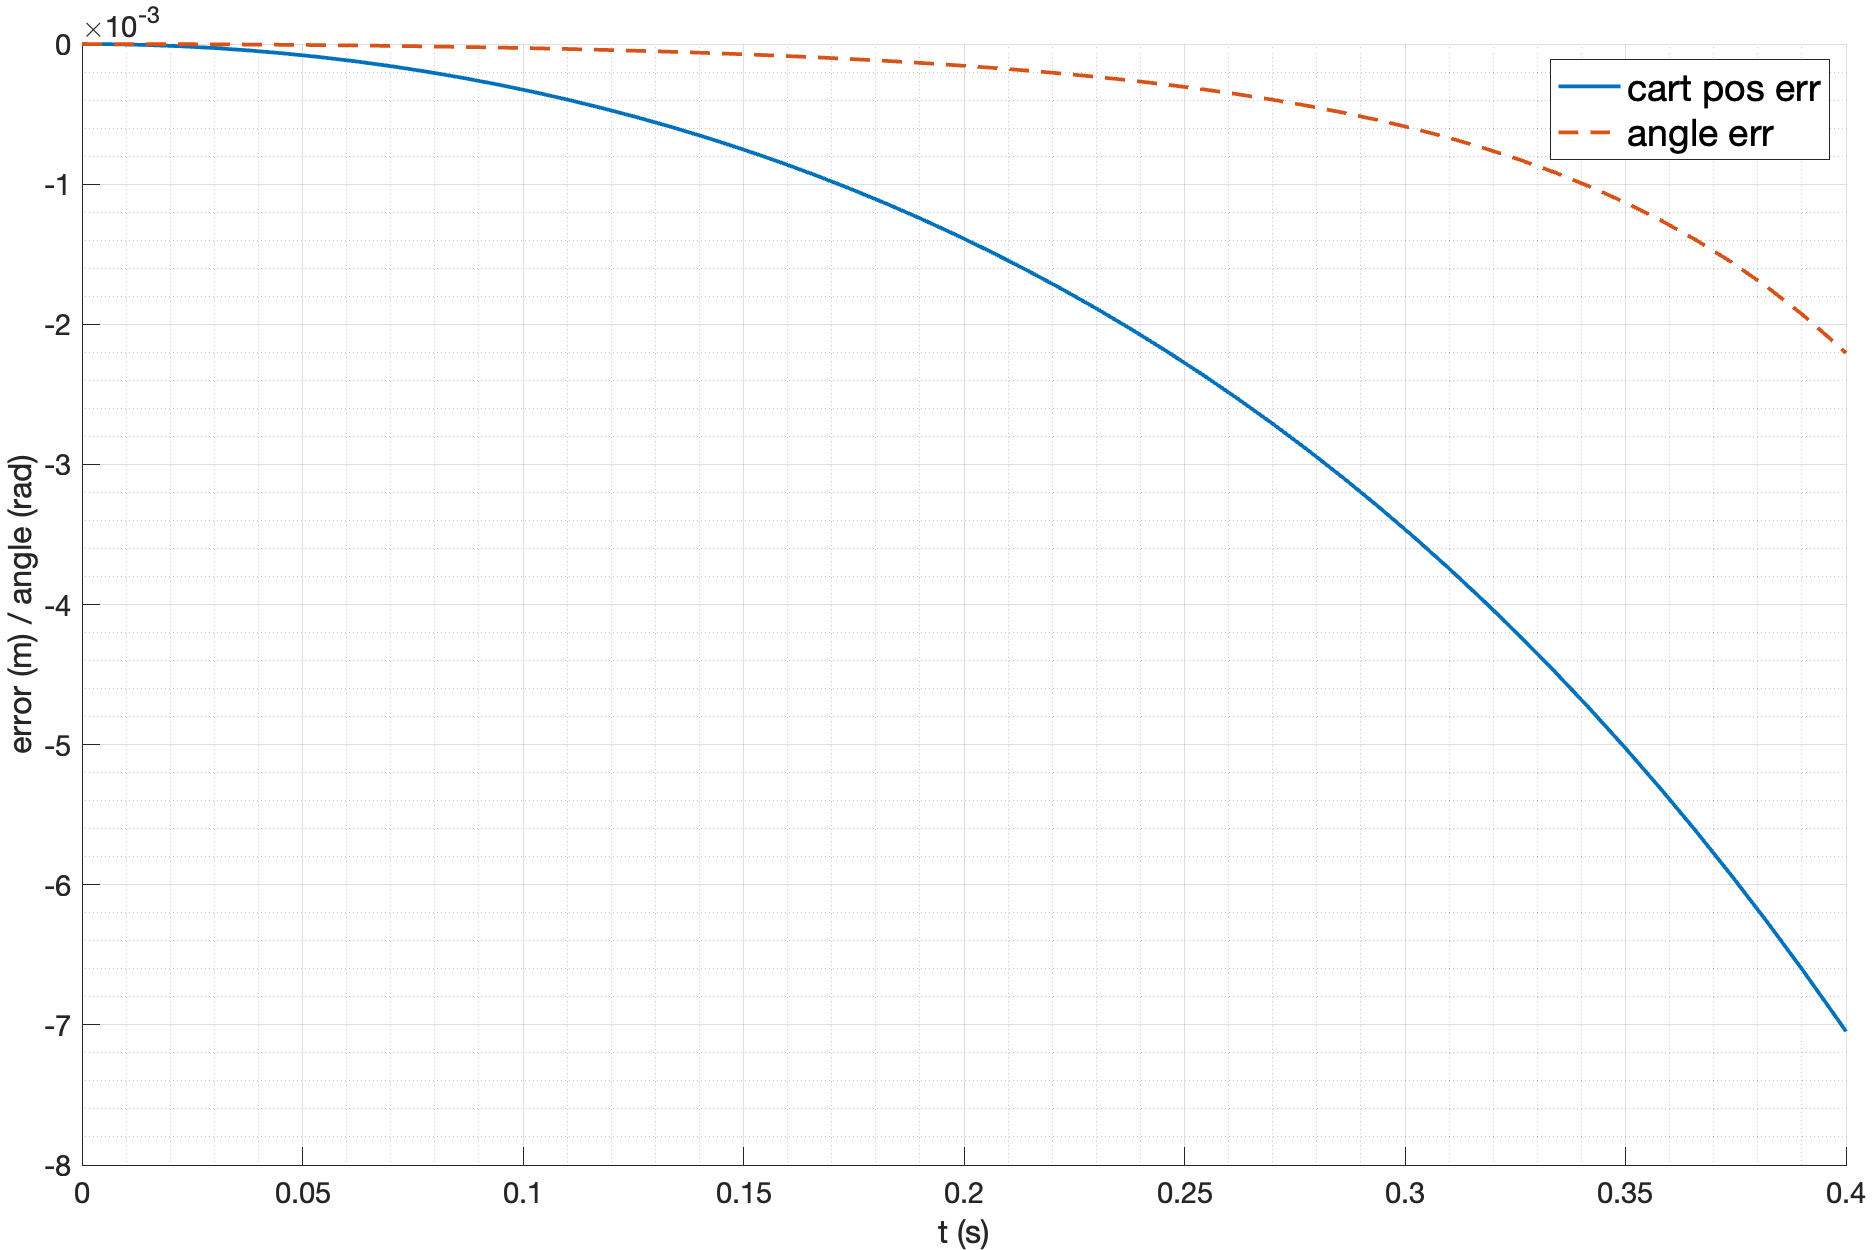
\includegraphics[width=\textwidth]{media/plots/free_motion/err_2.png}
        \caption{$\theta_0 = 0.1$}
    \end{subfigure}
    \begin{subfigure}[b]{0.45\textwidth}
        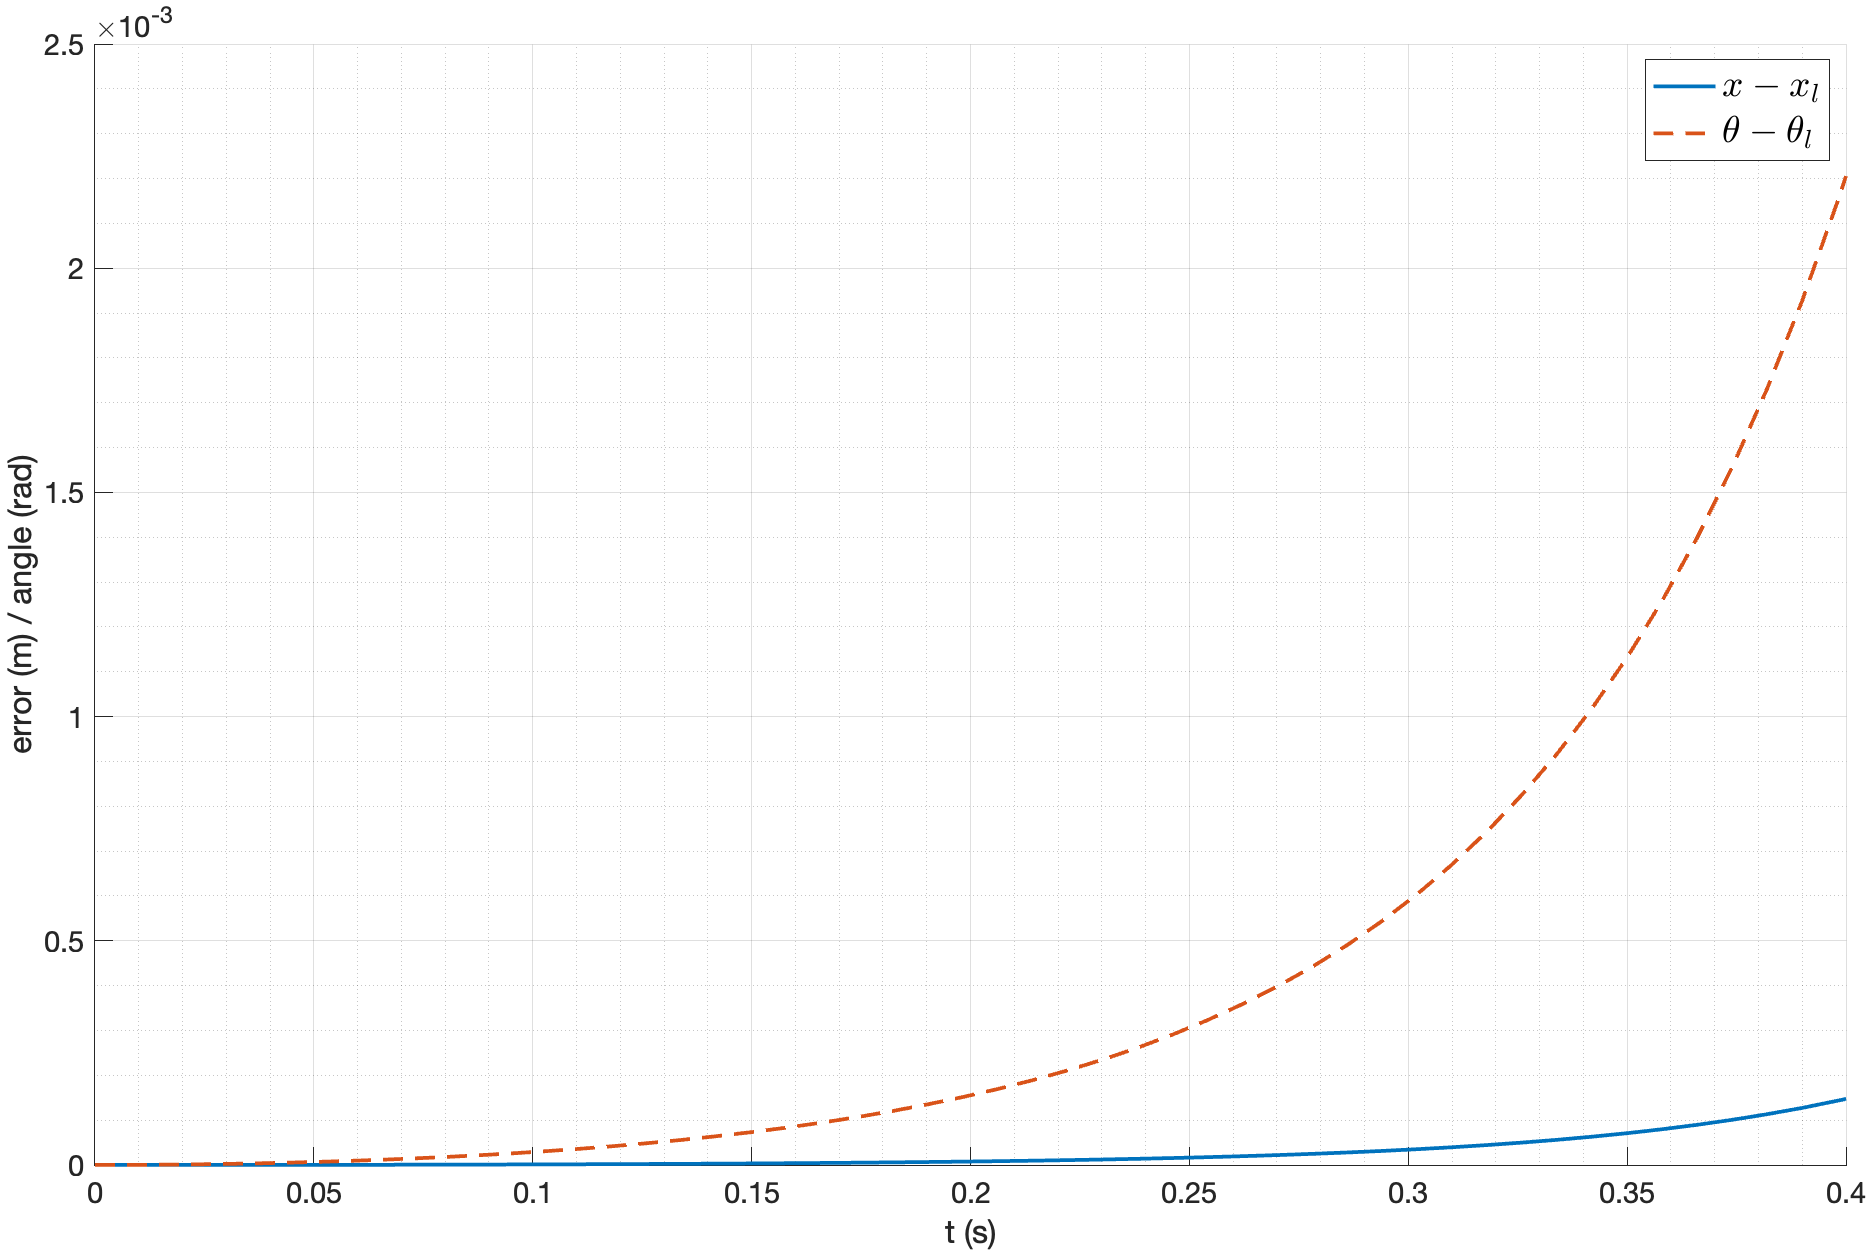
\includegraphics[width=\textwidth]{media/plots/free_motion/err_3.png}
        \caption{$\theta_0 = -0.1$}
    \end{subfigure}
    \begin{subfigure}[b]{0.45\textwidth}
        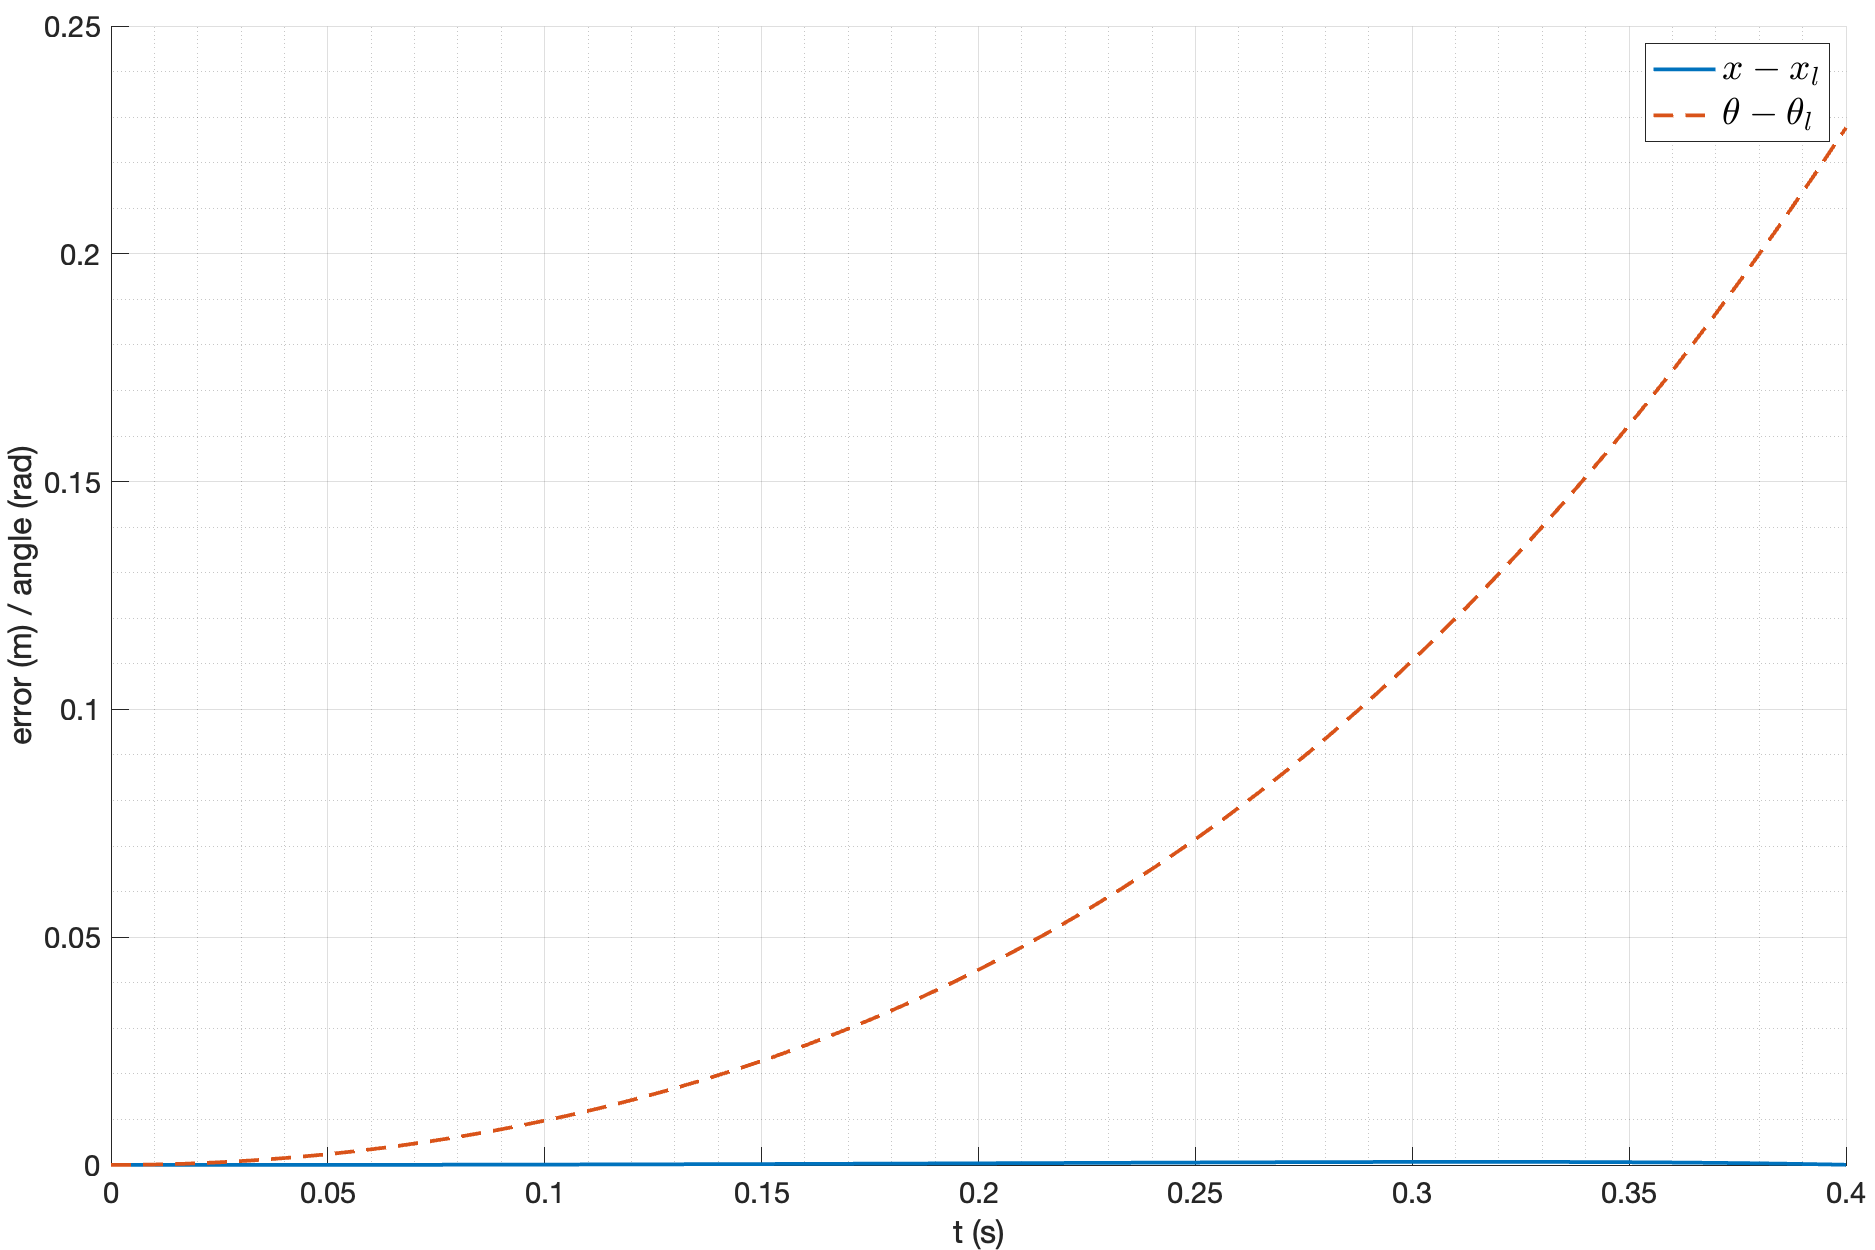
\includegraphics[width=\textwidth]{media/plots/free_motion/err_4.png}
        \caption{$\theta_0 = 0.3$}
    \end{subfigure}
    \begin{subfigure}[b]{0.45\textwidth}
        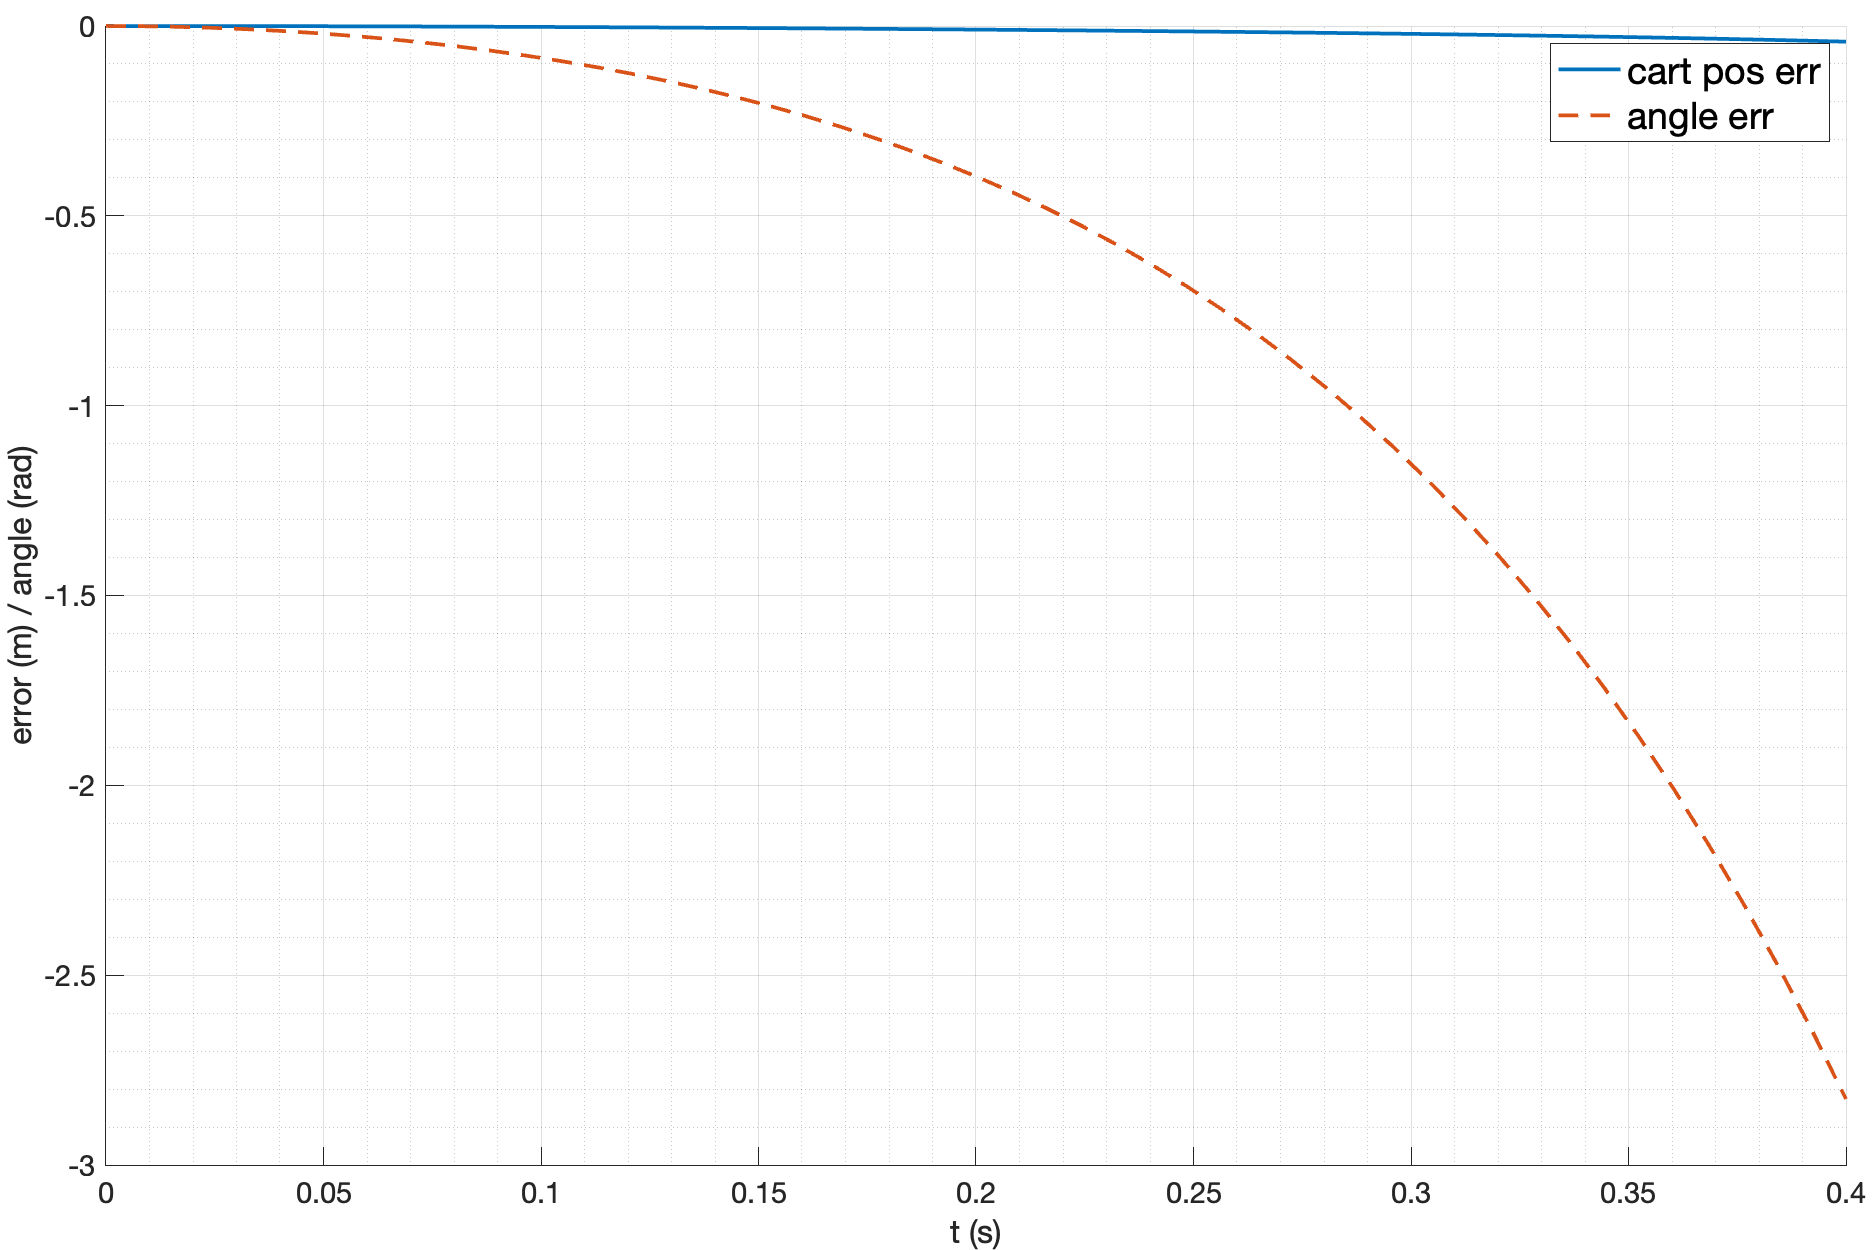
\includegraphics[width=\textwidth]{media/plots/free_motion/err_5.png}
        \caption{$\theta_0 = \frac{\pi}{2}$}
    \end{subfigure}
    \begin{subfigure}[b]{0.45\textwidth}
        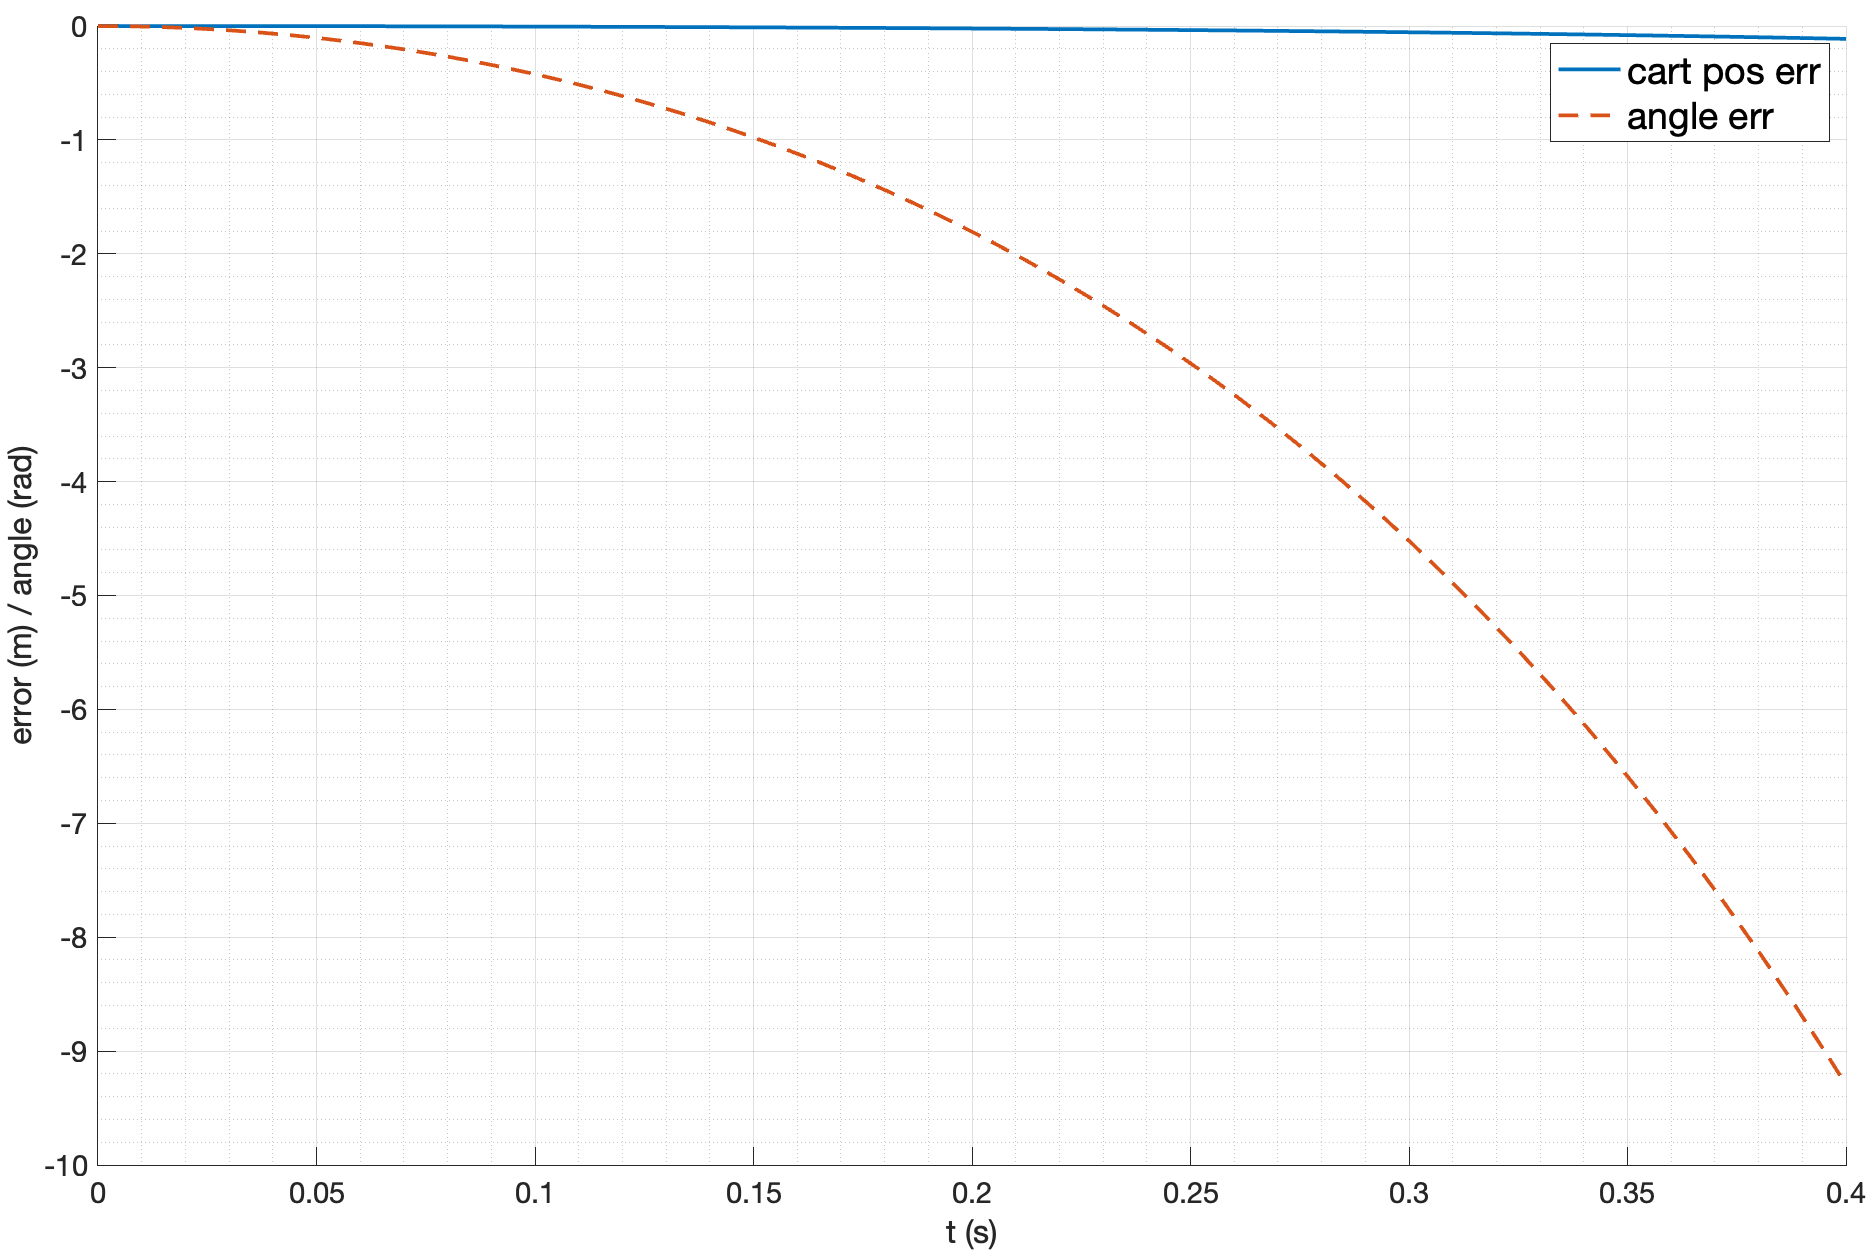
\includegraphics[width=\textwidth]{media/plots/free_motion/err_6.png}
        \caption{$\theta_0 = \pi$}
    \end{subfigure}
    \caption{Различия в движении маятника (нелинейная и линеаризованная модели)}
    \label{fig:free_motion_err}
\end{figure}

Видно, что при отклонениях $\theta_0 = 0.1$, $\theta_0 = -0.1$ и $\theta_0 = 0.3$ 
различия в движении незначительны, при этом увеличиваются с увеличением 
модуля отклонения. При отклонении $\theta_0 = \frac{\pi}{2}$ различия в движении
уже становятся существенными, что, опять же, связано с линеаризацией вблизи 
верхней точки равновесия. 

Проведем моделирование системы с начальным отклонением $\theta_0 = 0.1$ на более длительном 
промежутке времени. Результаты моделирования представлены на рисунке \ref{fig:free_motion_long_linear}, 
\ref{fig:free_motion_long_nonlinear}. 
\begin{figure}[ht!]
    \centering
    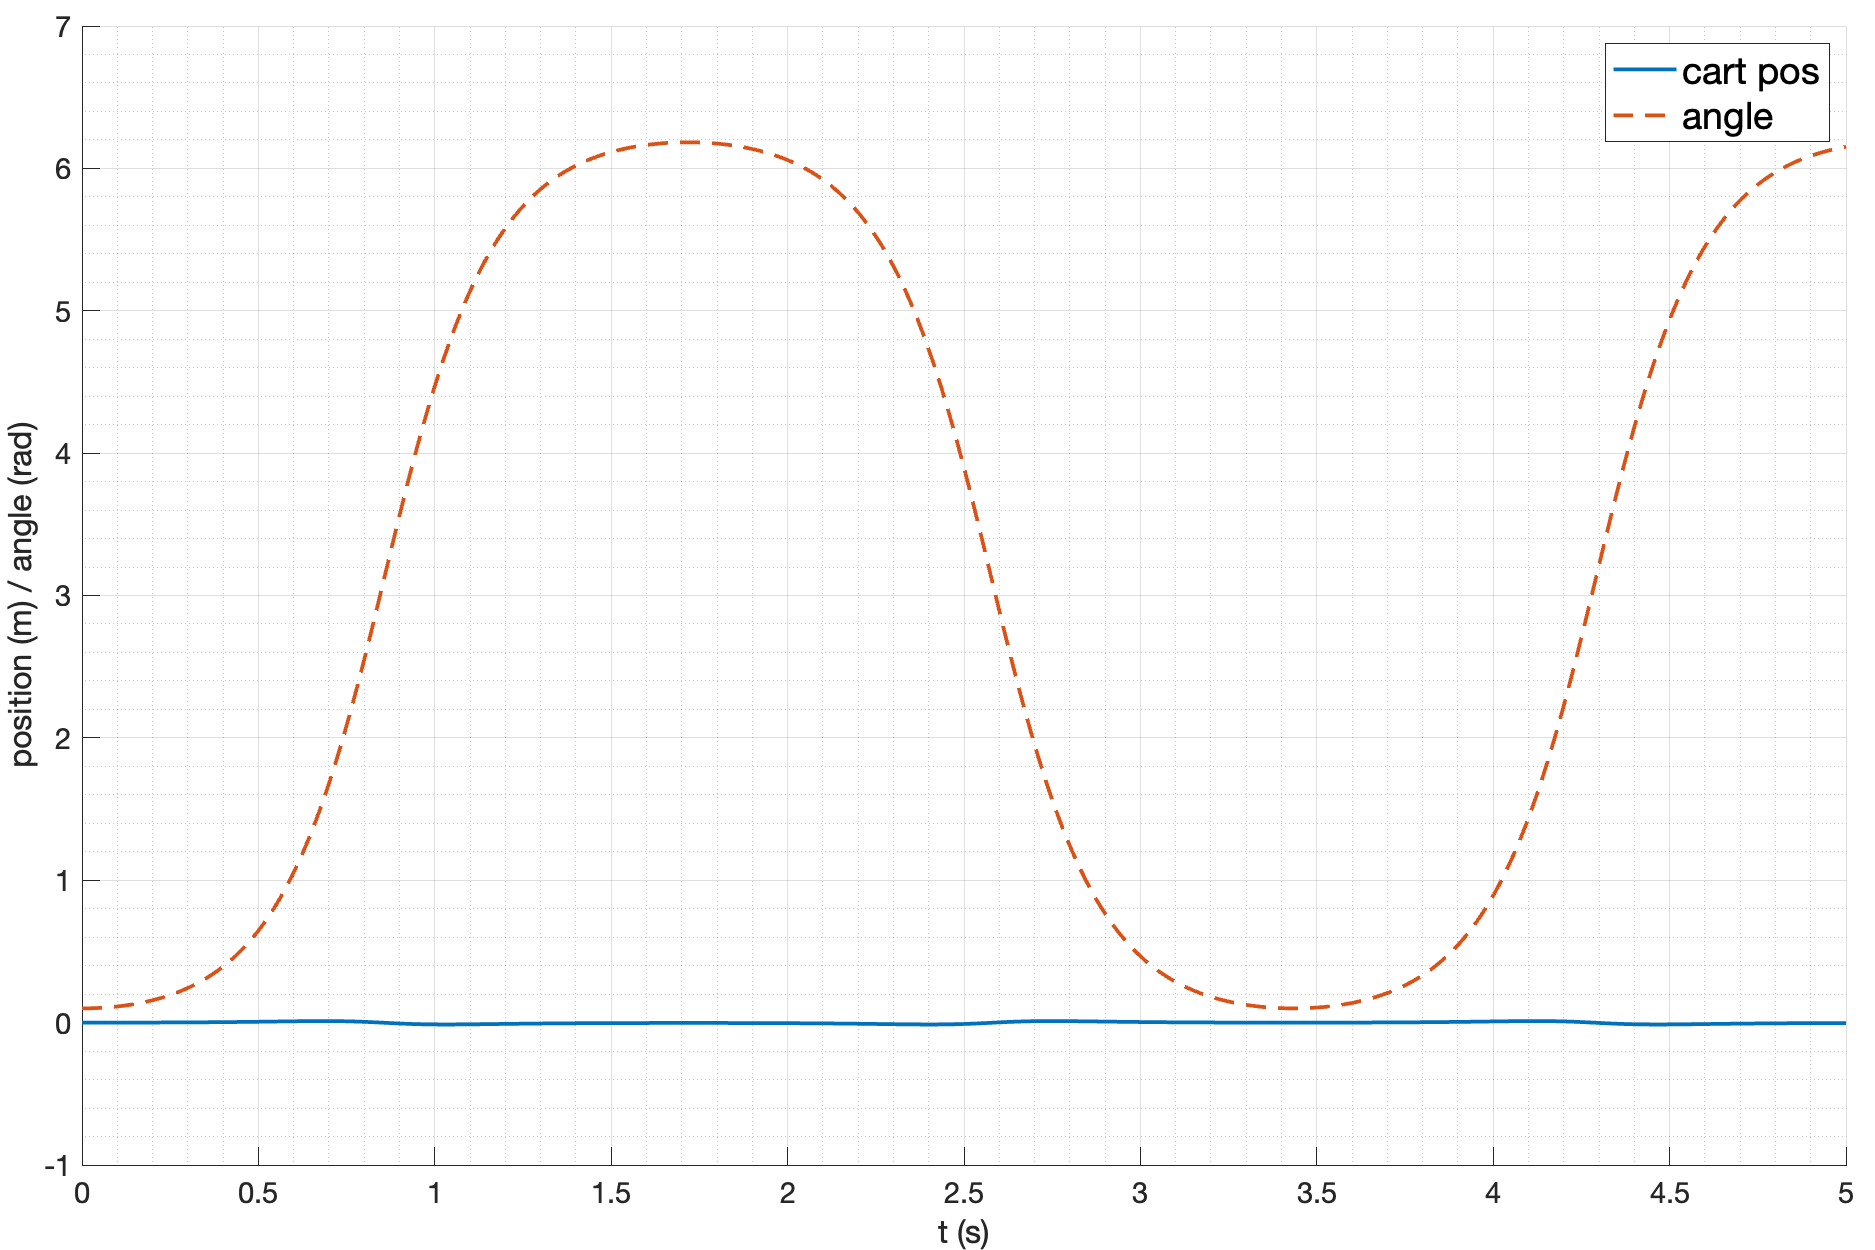
\includegraphics[width=\textwidth]{media/plots/free_motion/long.png}
    \caption{Свободное движение маятника (нелинейная модель)}
    \label{fig:free_motion_long_nonlinear}
\end{figure}
\begin{figure}[ht!]
    \centering
    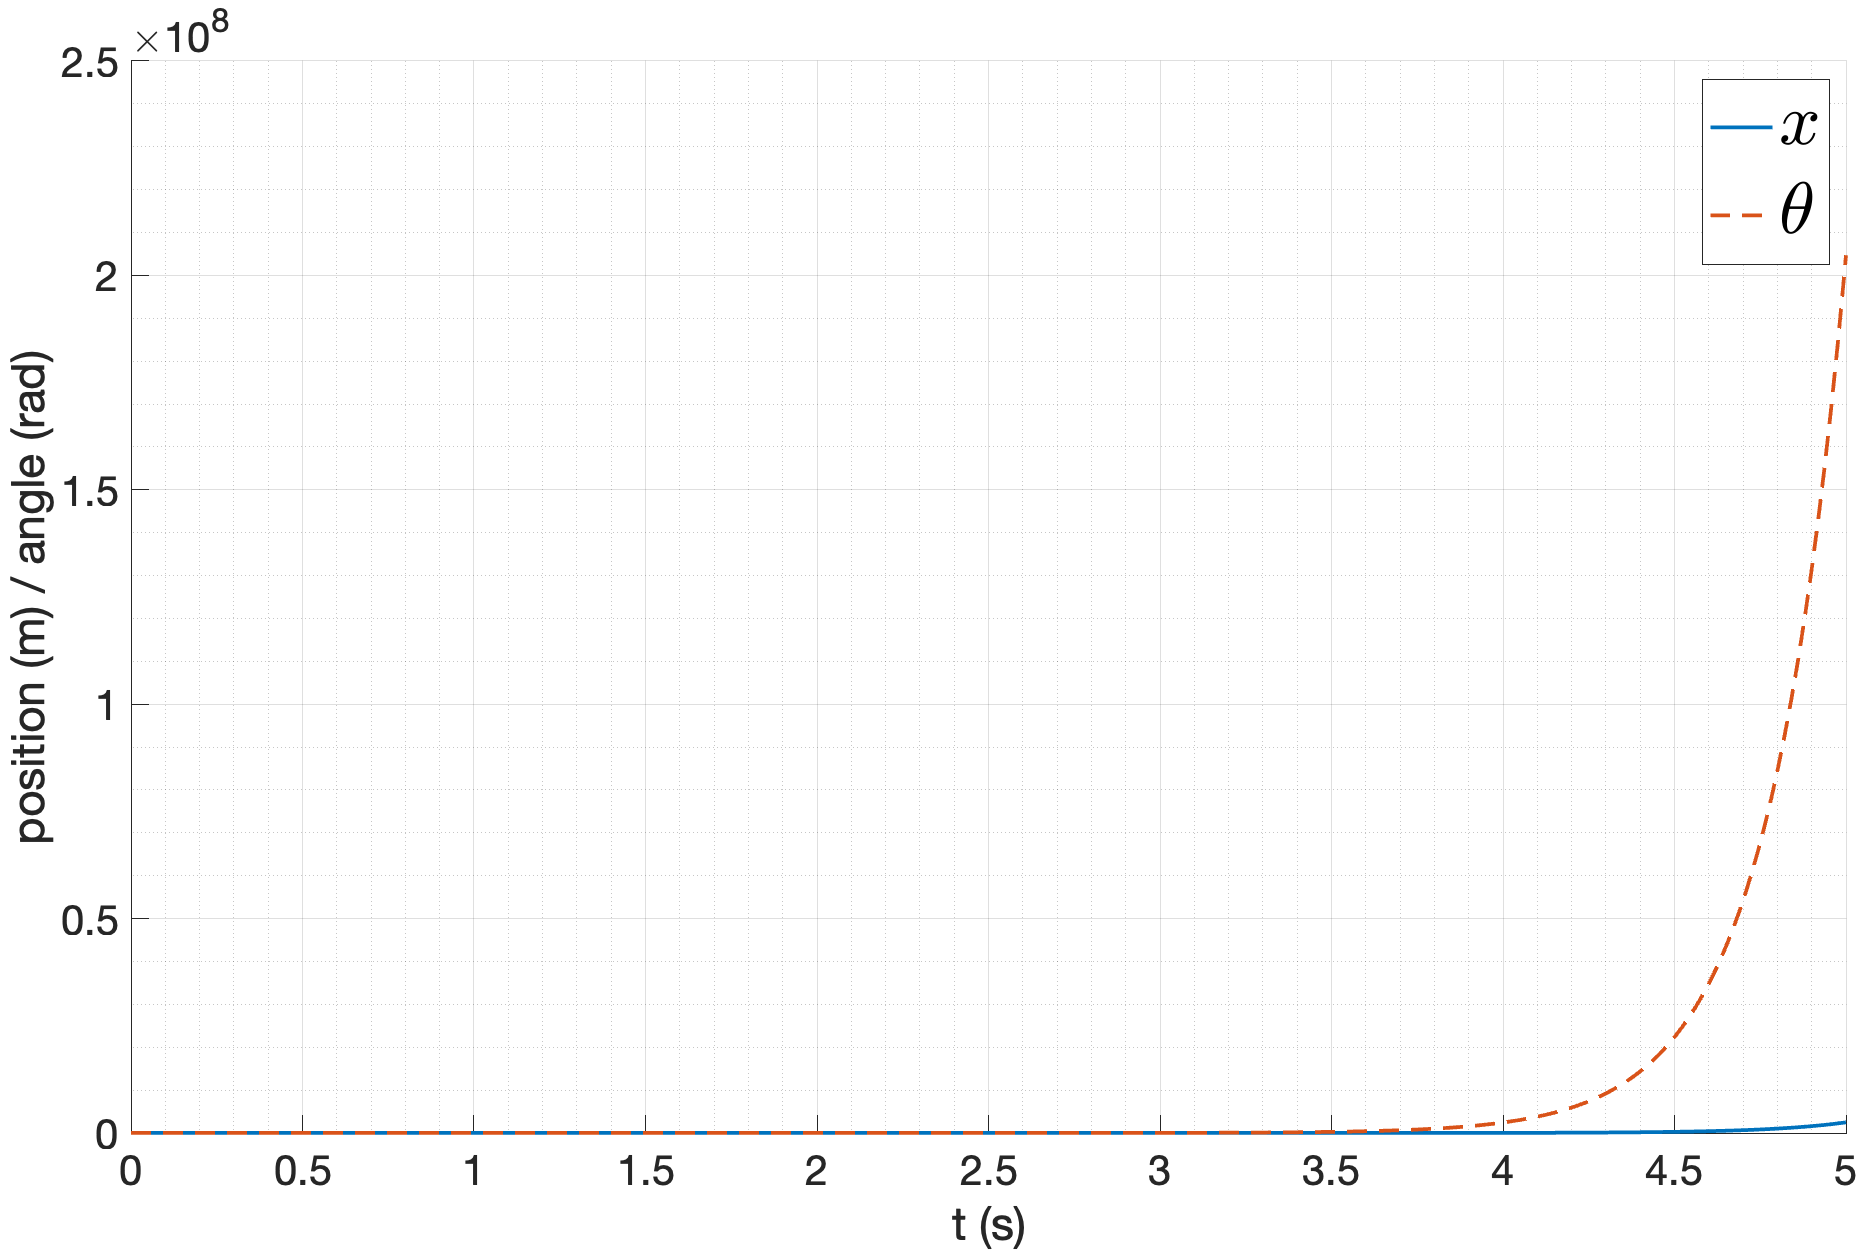
\includegraphics[width=\textwidth]{media/plots/free_motion/long_linear.png}
    \caption{Свободное движение маятника (линеаризованная модель)}
    \label{fig:free_motion_long_linear}
\end{figure}

На графиках \ref{fig:free_motion_long_nonlinear} и \ref{fig:free_motion_long_linear} видно, что
в случае нелинейной модели система колебалась с затухающими колебаниями, что является
ожидаемым результатом движения маятника, в то время как в случае линеаризованной модели система 
не является колебательной и выход системы стремится к бесконечности, это связано с тем, что
линеаризованная модель способна давать корректные результаты только в окрестности 
верхней точки равновесия, а при больших отклонениях от вертикального положения ее поведение
уже не является корректным.

\FloatBarrier
\subsubsection{Итоги моделирования}
В ходе анализа и моделирования модели системы перевернутого маятника на тележке 
и ее линеаризованной модели при небольших отклонениях от вертикального положения 
было показано, что линейная модель является хорошим приближением нелинейной модели 
в окрестности верхней точки равновесия, что позволяет использовать ее для дальнейшего
синтеза. Можно, изменив способ задания угла отклонения, получить линейную модель, 
описывающую движение маятника в окрестности нижней точки равновесия, что 
может быть использовано для создания модели козлового крана.

Из-за того, что линеаризованная модель дает корректные результаты только в окрестности 
верхней точки равновесия, асимптотическое ее поведение сильно отличается от
асимптотического поведения нелинейной модели, так же как в случае 
существенных отклонений от вертикального положения. 